\documentclass[12pt,a4paper,titlepage]{vorkurs}

\fancyhf{}
\fancyhead[C]{Vorkurs (Mathematik)}
\fancyhead[L]{\leftmark}
\renewcommand{\headrulewidth}{0.5 pt}
\fancyfoot[L]{\today}
\fancyfoot[C]{\thepage}
\fancyfoot[R]{FS07}
\usepackage[utf8]{inputenc}
\begin{document}
\pagenumbering{roman}
\titlehead
{
 	\begin{flushright}
 		\includegraphics[width = 7cm]{pictures/hm-logo}
 	\end{flushright}
 	 	\line(1,0){400}
}

\subject{\includegraphics*[width=9 cm]{pictures/fs-logo}}
\title{Vorkurs /Mathematik}
\subtitle{Eine Wiederholung des mathematischen Schulstoffs}
\author{by Stephan Pl"oderl}
\publishers{Fachschaft 07}
\date{\today}
\thispagestyle{empty}
\maketitle
\newpage
\setcounter{page}{1}
\tableofcontents
\newpage
\clearpage

\pagenumbering{arabic}
\psection{Einf"uhrung}
\subsection{Worum geht's im Vorkurs Mathematik?}
Jeder Studierende tut sich in unterschiedlichen F"achern unterschiedlich schwer.
Es gibt jedoch F"acher, in denen die Durchfallquote bereits "uber Jahre "uberdurchschnittlich hoch ist.
Bei einem dieser F"acher mit besonders hoher Durchfallquote handelt es sich um das mathematische Fach Analysis.
Aus diesem Grund haben wir als Fachschaft es uns so wie bereits einige vor uns zur Aufgabe gemacht, dem ganzen ein wenig entgegenzusteuern und zu versuchen, euch die Grundlagen die f"ur dieses Fach von N"oten sind zu vermitteln.

\subsection{An wen richtet sich dieser Kurs?}
Dieser Kurs richtet sich an all jene,
\begin{itemize}
\item welche Schwächen in mathematischen F"achern haben.
\item deren Schulzeit schon etwas länger her ist.
\item welche nicht von mathematisch/technischen Schulen bzw. Gymnasien kommen.
\item und an all jene welche der Meinung sind, eine Wiederholung schadet nie.
\end{itemize}

\subsection{Warum Mathematik im Informatikstudium?}
Vor allem in den ersten Semestern stehen die Mathematikvorlesungen im Informatikstudium (Scientific Computing, Wirtschaftsinformatik, Geotelematik) immer etwas Abseits. Vielen Studierenden ist nicht klar, warum Mathematik so grundlegend wichtig f"ur ihr Studium ist - schlie"slich studieren sie ja keine (reine) Mathematik! Dieses Kapitel soll dieses Verst"andnisproblem l"osen und aufzeigen, welche Schnittpunkte zwischen Mathematik und Informatik bestehen. Es ist n"amlich keineswegs so, dass Mathematik immer die graue, langweilige Theorie ist, die \glqq durchgestanden werden muss\grqq ! Mit Mathematik haben Informatiker ein zus"atzliches, sehr m"achtiges Werkzeug zur Hand, mit dem viele scheinbar unl"osbare Probleme (in der Informatik!) pl"otzlich l"osbar werden. Das tolle ist: Man muss nicht erst die komplette Mathematik verstanden haben, um sie als Werkzeug verwenden zu k"onnen. Es gilt eher der Grundsatz: Mehr hilft mehr! In manchen Bereichen ist allerdings ein Grundverst"andnis notwendig, um sich das Werkzeug auch wirklich zu Nutze machen zu k"onnen. Einige dieser Bereiche versucht dieses Kapitel anzusprechen.

Zumindest grundlegende Mathematikkenntnisse sind in den folgenden Informatikbereichen wichtig. Diese Liste ist nicht vollst"andig und gibt nur einen kleinen Ausschnitt wider:
\begin{itemize}
\item Spieleentwicklung
\item Physiksimulationen
\item Supercomputing
\item Robotik
\item Business Analytics
\item Data Mining
\item Machine Learning
\end{itemize}
%Comment: Überflüssig, das sieht der Leser ja?
%Die Themen Spieleentwicklung, Business Analytics und Machine Learning werden im folgenden Text als Beispiele verwendet, dass Mathematik auch als Werkzeug f"ur Informatiker sehr n"utzlich ist.

\subsubsection{Spieleentwicklung}
Die Entwicklung eines Spiels umfasst neben Informatik noch sehr viele andere Bereiche: Design, Architektur, Psychologie, Soziologie, Teamf"uhrung, Finanzierung, Marketing und Musik sind alle in mehr oder weniger gro\ss em Umfang f"ur ein gutes Spiel n"otig. Die Mathematik ebenfalls: sobald sich ein Spielelement zumindest halbwegs realistisch bewegen soll, m"ussen die entsprechenden Bewegungsgleichungen (numerisch) integriert werden. Auch Lichteffekte wie Spiegelungen oder der Soundeffekte wie Widerhall m"ussen zuerst korrekt mathematisch beschrieben und dann implementiert werden, wenn sie \glqq echt\grqq aussehen sollen. Daneben sind auch Performanceprobleme zu l"osen: zum Beispiel wurde im Spiel \emph{Quake} eine schnelle Wurzelberechnung verwendet, ohne die alles unspielbar langsam geworden w"are. (Zur Implementierung siehe \url{http://www5.in.tum.de/lehre/vorlesungen/konkr_math/SS_15/prog/NumPro_SS15_Programmieraufgabe_1.pdf})
Alle beschriebenen Probleme k"on\-nen mit relativ einfachen, mathematischen Methoden gel"ost werden - diese k"onnen alle im Studium gelernt werden (Analysis, Lineare Algebra, Numerik, Integraltransformationen, Differentialgleichungen, Algorithmen und Datenstrukturen).

\subsubsection{Business Analytics}
Der Begriff \glqq Big Data\grqq ist in den letzten Jahren immer gebr"auchlicher geworden - Unternehmen versuchen aus gro\ss en Datenmengen, die sie "uber ihre Kunden sammeln, Informationen und Wissen zu generieren. Dieses Wissen soll dann in Verbesserung von Produkten oder in neue Produkte umgesetzt werden, die verkauft werden k"onnen. Business Analytics ist ein Teilgebiet von Data Mining, das speziell die Probleme in der Unternehmenswelt mittels Datenanalyse zu l"osen versucht. Solche Probleme sind zum Beispiel die Ermittlung von \glqq Risikokunden\grqq von Handyvertr"agen, die unzufrieden sind und deshalb k"undigen wollen. K"onnen diese Kunden per Business Analytics gezielt ermittelt werden, werden ihnen Sonderangebote wie kostenlose Freiminuten geschenkt - mit dem Ziel, dass sie den Vertrag weiterlaufen lassen. Die Ermittlung der Kunden erfolgt durch statistische Analysen wie Regression oder Decision Trees - also alles wieder mathematische Werkzeuge, die im Studium erlernt werden k"onnen (Lineare Algebra, Wahrscheinlichkeitstheorie und Statistik).

\subsubsection{Machine Learning}
Durch die immer schneller rechnenden Computer k"onnen heute Probleme gel"ost werden, die fr"uher nur Menschen erledigen konnten. Dazu geh"oren automatische Gesichtserkennung, das Auffinden von Tumoren in medizinischen Bildern oder die Erkennung von Kreditkartenbetrug. Meist steht hinter diesen Anwendungen das sogenannte \glqq Machine Learning \grqq, was bedeutet, dass die Maschine (der Computer) selbst lernt, welche Eigenschaften in den auftretenden Daten (Bilder von Gesichtern, Kreditkarten"uberweisungen, Bilder von Tumoren oder gesundem Gewebe) zu welchem Ergebnis passt (Gesichter werden bestimmten Menschen zugeordnet, eine "uberweisung wird als Betrug markiert, ein Gewebebild wird als gesund gekennzeichnet). Das praktische am selbstlernenden Computer: der Mensch muss nur noch eine sogenannte Trainingsmenge an Datenmaterial bereitstellen, an der der Computer lernen kann - nach dem Training ist die Maschine selbst"andig in der Lage, eine Zuordnung zu machen - es ist also nicht n"otig, in m"uhevoller Kleinarbeit selbst die Eigenschaften eines Tumors oder eines Kreditkartenbetrugs herauszufinden und sie die entsprechende Software zu schreiben.
Die selbstlernenden Programme sind allerdings selbst von Menschen geschrieben und enthalten teilweise viel, teilweise aber auch relativ wenig Mathematik - es gibt allerdings keins, das komplett ohne mathematische Grundlagen in der Praxis gut funktioniert. Die sogenannten \glqq neuronalen Netze\grqq \ (\url{https://en.wikipedia.org/wiki/Artificial_neural_network}) funktionieren im Hintergrund mit Ma\-trix/\-Vektor-\-Multiplikationen, die schon im ersten Semester in Linearer Algebra gelernt werden k"onnen. Weitere Techniken wie Regression, Bildverarbeitung oder Filterungen k"onnen in weiterf"uhrenden, mathematischen F"achern erlernt werden und setzen auf die Grundlagen in Analysis (Integration, Differentiation, Funktionen) und Linearer Algebra (Matrizenrechnung) auf.

\subsubsection{Mathematik - Weg zum Verst"andnis}
Auch wenn sie sehr praktisch anwendbar ist - Mathematik ist weit mehr als nur ein Werkzeug zur L"osung von Ingenieursproblemen. Wer sich genauer damit befasst wird merken, dass sich nach und nach der eigene Geist ver"andert. Man wird kritischer, hinterfragt viele Dinge des normalen Lebens und kann Probleme (nicht nur mathematische!) viel klarer angehen als ohne mathematische Ausbildung. Den eigenen Geist zu ver"andern ist allerdings eine unglaublich schwierige Angelegenheit, weil man st"andig gegen eigene Widerst"ande zu k"ampfen hat. Das wird schon bei den "Ubungsaufgaben im Studium ersichtlich, die teilweise einfach nicht klappen wollen - und zwar so lange, bis das Verst"andnis des Themas einsetzt. Auf einmal sieht die L"osung dann einfach aus, und genau in diesem Moment sollte man kurz dar"uber nachdenken, dass sich gerade der eigene Geist ver"andert hat. Man hat etwas dazugelernt, was kein Faktenwissen ist, sondern eine neue Art Probleme zu l"osen: echtes Verst"andnis.
Wer hier interessiert ist, dem empfehlen wir die Lekt"ure des folgenden Artikels: \url{http://arxiv.org/abs/math/9404236}.


\psection{Logik}
Die Logik öffnete den Weg für die Informatik. Sie war immer eine Disziplin der Philosophie und hat eine sehr interessante Geschichte (von Aristoteles, Kant, Hegel, Boole, Russell, Gentzen, Skolem, Gödel, bis zu Turing und weiter) hinter sich gelassen. Die Aussagenlogik, als kleiner aber grundlegender Teil, ist fundamental um mathematische Ausdrücke zu verstehen und wird in allen Bereichen der Mathematik verwendet.
\begin{warning}
In der Informatik hat die Logik eine wichtige Bedeutung. In der technischen Informatik werden Recheneinheiten mit sogenannten logischen Gattern realisiert. Ein Gatter ist nichts anders als eine logische Verknüpfung. Zum Beispiel ist das Und-Gatter ein Gatter mit zwei Eingängen $x_{in}^1, x_{in}^2$ und einem Ausgang $x_{out}$.\\
Legt man nun Spannung an $x_{in}^1$ und \textit{gleichzeitig} $x_{in}^2$ an, so gibt das Gatter diese Spannung weiter, ansonsten nicht. Die Gatter bilden den Kern der Computerhardware wie z.B. Mikroprozessoren. Zudem ist die Aussagenlogik in jeder Programmiersprache eingebettet.
\end{warning}

\subsection{Aussagenlogik}
\begin{definition}[Aussage]
Eine Aussage ist ein als Satz formulierter Gedanke, dem man auf sinnvolle Weise einen Wahrheitswert zuordnen kann.
\end{definition}
%\begin{axiom}[Gesetz vom ausgeschlossenen Dritten]
Eine Aussage ist entweder \textbf{wahr (w)} oder \textbf{falsch (f)} (Gesetz vom ausgeschlossenen Dritten).
%\end{axiom}

\subsubsection*{Beispiele}
\begin{itemize}
\item $A_1 := $ Die Sonne strahlt wärme ab.
\item $A_2 := $ Bayern München wird diese Saison wieder deutscher Meister.
\item $A_3 := 1+1 = 2$
\item $A_4 := $ Wird in diesem Jahr Ostern gefeiert?
\end{itemize}
$A_1$ und $A_3$ sind offensichtlich wahre Aussagen. $A_2$ können wir derzeit nicht überprüfen, sie ist aber trotzdem wahr oder falsch und darum zulässig. $A_4$ ist keine Aussage, sondern eine Frage - die Antwort darauf kann wieder eine Aussage sein (z.B. \textit{In diesem Jahr wird Ostern gefeiert.}).

\subsubsection*{Schreibweisen}
Wir schreiben gewöhnlich $A$ ist \textbf{wahr} oder \textbf{falsch}, \textbf{w} oder \textbf{f} bzw. (für uns Informatiker) \textbf{1} oder \textbf{0}.

\subsubsection{Logische Verknüpfungen}
\begin{definition}[Negation]
Unter der Negation einer Aussage $A$ versteht man die Aussage $\neg A$ (Mathe) bzw. $\overline{A}$ (Informatik) (in Worten:\glqq nicht $A$\grqq ), die genau dann wahr ist, wenn $A$ selbst falsch ist.
\end{definition}
Es folgt eine sogenannte \textbf{Wahrheitstabelle} der Verknüpfung. In der ersten Spalte stehen die Werte, die $A$ annimmt, und in der rechten Spalte, Werte, die $\neg A$ dann besitzt.
\begin{center}
\begin{tabular}{c||c}
 $A$ & $\neg A$  \\ 
\hline
\cellcolor{ared}falsch  & \cellcolor{agreen}wahr   \\ 
\cellcolor{agreen}wahr  & \cellcolor{ared} falsch  \\ 
\hline
\end{tabular}
\end{center}

\paragraph*{Beispiel:}
\begin{itemize}
	\item Die Negation der Aussage \glqq 4 ist ungerade\grqq \ ist die Aussage \glqq 4 ist gerade\grqq , denn es gibt nur diese beiden Möglichkeiten.
	\item Aber die Negation der Aussage \glqq 4.5 ist ungerade\grqq \ ist nicht die Aussage \glqq 4.5 ist gerade\grqq, denn beide Aussagen sind falsch, ja sogar unsinnig. Die Negation der Aussage \glqq Diese Kuh ist schwarz\grqq \ ist nicht etwa die Aussage \glqq Diese Kuh ist weiß\grqq , denn es gibt ja noch andere Farben. Vielmehr müsste man sagen:\glqq Diese Kuh ist nicht schwarz\grqq. Das umgangssprachliche Gegengenteil ist meist etwas anderes als die logische Verneinung.
\end{itemize}

\begin{definition}[Konjunktion]
Unter der Konjunktion zweier Aussagen $A$ und $B$ versteht man die Aussage $A \land B$ (Mathe) bzw. $A \cdot B$ (Informatik) (in Worten:\glqq $A$ und $B$\grqq ), die genau dann wahr ist, wenn $A$ und $B$ gleichzeitig wahr sind.
\end{definition}
In den ersten Spalten dieser \textbf{Wahrheitstabelle} stehen die Werte der Variablen der Konjunktion, in der letzten Spalte der resultierende Wert.
\begin{center}
\begin{tabular}{c|c||c}
 $A$& $B$  &  $A \land B$  \\ 
\hline
\cellcolor{ared} falsch & \cellcolor{ared} falsch & \cellcolor{ared} falsch   \\ 
\cellcolor{ared} falsch & \cellcolor{agreen} wahr & \cellcolor{ared} falsch  \\ 
\cellcolor{agreen} wahr & \cellcolor{ared} falsch & \cellcolor{ared} falsch   \\ 
\cellcolor{agreen} wahr & \cellcolor{agreen} wahr & \cellcolor{agreen} wahr  \\ 
\hline
\end{tabular}
\end{center}

\paragraph*{Beispiel:}
\begin{itemize}
	\item \glqq 18 ist eine gerade Zahl und durch 3 teilbar\grqq , ist eine wahre Aussage im Rahmen des Axiomensystems für die Arithmetik, welche hier umgangssprachlich vorausgesetzt wurde. Eigentlich handelt es sich um die Aussage \glqq 18 ist eine gerade Zahl, und 18 ist durch 3 teilbar\grqq .
	\item \glqq 15 ist eine gerade Zahl und durch 3 teilbar\grqq, ist eine falsch, denn der erste Teil der Aussage ist falsch.
\end{itemize}

\begin{definition}[Disjunktion]
Unter der Disjunktion zweier Aussagen $A$ und $B$ versteht man die Aussage $A \lor B$ (Mathe) bzw. $A + B$ (Informatik) (in Worten:\glqq $A$ oder $B$\grqq ), die genau dann wahr ist, wenn wenigstens eine der Aussagen $A$ oder $B$ wahr ist.
\end{definition}
In den ersten Spalten dieser \textbf{Wahrheitstabelle} stehen die Werte der Variablen der Disjunktion, in der letzten Spalte der resultierende Wert.
\begin{center}
\begin{tabular}{c|c||c}
$A$& $B$  &  $A \lor B$  \\ 
 \cellcolor{ared}falsch & \cellcolor{ared} falsch & \cellcolor{ared}falsch   \\ 
 \cellcolor{ared}falsch & \cellcolor{agreen}wahr & \cellcolor{agreen}wahr  \\ 
 \cellcolor{agreen}wahr & \cellcolor{ared} falsch & \cellcolor{agreen}wahr   \\ 
\cellcolor{agreen}wahr & \cellcolor{agreen}wahr & \cellcolor{agreen}wahr  \\ 
\hline
\end{tabular}
\end{center}
\begin{warning}
	Umgangssprachlich meinen wir mit \glqq oder\grqq \ meist \glqq entweder $\ldots$ oder\grqq . Was aber nicht der logischen Disjunktion entspricht.
\end{warning}

\paragraph*{Beispiel:}
\begin{itemize}
	\item \glqq Ich werde Mathematik oder Informatik studieren\grqq , diese Aussage ist auch dann wahr, wenn ich mich dafür entscheide, beide Fächer zu studieren. Falsch wird sie aber z.B., wenn ich nur Biologie studiere.
	\item \glqq Ich kann nur Hü oder Hott sagen\grqq . Das ist natürlich falsch, denn ich kann ja beide Wörter vermeiden.
\end{itemize}

\begin{definition}[Implikation]
Unter der Implikation zweier Aussagen $A$ und $B$ versteht man die Aussage $A \Rightarrow B$ (in Worten:\glqq $A$ impliziert $B$\grqq oder \glqq aus $A$ folgt $B$\grqq ), versteht man die Zusammengesetzte Aussage $ (\neg A) \lor B$.
\end{definition}
In den ersten Spalten dieser \textbf{Wahrheitstabelle} stehen die Werte der Variablen der Implikation, in der letzten beiden Spalte der resultierenden Werte (in der letzten der finale Wert).
\begin{center}
\begin{tabular}{c|c||c||c}
$A$& $B$ &$\neg A$&  $\neg A \lor B$  \\ 
 \cellcolor{ared}falsch &  \cellcolor{ared}falsch & \cellcolor{agreen}wahr  & \cellcolor{agreen}wahr  \\ 
 \cellcolor{ared}falsch & \cellcolor{agreen}wahr & \cellcolor{agreen}wahr  &  \cellcolor{agreen}wahr  \\ 
\cellcolor{agreen}wahr &  \cellcolor{ared}falsch & \cellcolor{ared} falsch  &  \cellcolor{ared}falsch  \\ 
\cellcolor{agreen}wahr & \cellcolor{agreen}wahr & \cellcolor{ared} falsch  &  \cellcolor{agreen}wahr  \\ 
\hline
\end{tabular}
\end{center}

$A$ wird auch als Prämisse bezeichnet. Eigentlich sieht alles recht einfach aus. Nehmen wir die Aussagen: ($A$) \glqq Wenn es regnet folgt daraus, dass ($B$) die Stra{ß}e nass wird\grqq . Wenn es nun regnet und die Stra{ß}e nass wird ist die Aussage wahr. Doch was passiert wenn es nicht regnet?\\
Wenn es nicht regnet ist die Aussage immer wahr egal ob die Stra{ß}e nun nass oder trocken ist.
Wir können die Aussage auch wie folgt formulieren:
\begin{center}
\glqq Ist die Stra{ß}e nicht nass, so folgt daraus, dass es nicht regnet.\grqq\\ (Kontropositionsgesetz)
\end{center}
\begin{equation*}
((\neg B) \Rightarrow (\neg A)) \iff (A \Rightarrow B)
\end{equation*}

\begin{definition}["Aquivalenz]
Unter der "Aquivalenz zweier Aussagen $A$ und $B$ versteht man die Aussage $A \iff B$ (in Worten:\glqq $A$ gilt genau dann wenn $B$ gilt\grqq ). Diese ist genau dann wahr wenn $A \Rightarrow B \land B \Rightarrow A$ wahr ist. 
\end{definition}
In den ersten Spalten dieser \textbf{Wahrheitstabelle} stehen die Werte der Variablen der "Aquivalenz, in der letzten Spalte der resultierende Wert.
\begin{center}
\begin{tabular}{|c|c||c|}
 $A$ & $B$ & $A \iff B$  \\ 
\cellcolor{ared}falsch & \cellcolor{ared}falsch & \cellcolor{agreen}wahr    \\ 
\cellcolor{ared}falsch & \cellcolor{agreen}wahr & \cellcolor{ared}falsch    \\ 
\cellcolor{agreen}wahr & \cellcolor{ared}falsch & \cellcolor{ared}falsch    \\ 
\cellcolor{agreen}wahr & \cellcolor{agreen}wahr & \cellcolor{agreen}wahr    \\ 
\hline
\end{tabular}
\end{center}
Ein Beispiel wäre $x + 5 = 7 \iff x + 8 = 10$.


\begin{definition}[Exklusives Oder]
Unter dem exklusives Oder zweier Aussagen $A$ und $B$ versteht man die Aussage $A \text{ XOR } B$ (in Worten:\glqq entweder $A$ oder $B$\grqq ). Diese ist genau dann wahr wenn $(A \land \neg B) \lor (\neg A \land B)$ wahr ist. 
\end{definition}
In den ersten Spalten dieser \textbf{Wahrheitstabelle} stehen die Werte der Variablen des exklusiven Oder, in der letzten Spalte der resultierende Wert.
\begin{center}
\begin{tabular}{|c|c||c|}
$A$ & $B$ & $A \textsf{ XOR } B$  \\ 
\cellcolor{ared}falsch &  \cellcolor{ared}falsch &  \cellcolor{ared}falsch    \\ 
\cellcolor{ared}falsch & \cellcolor{agreen}wahr & \cellcolor{agreen}wahr    \\ 
\cellcolor{agreen}wahr & \cellcolor{ared}falsch & \cellcolor{agreen}wahr    \\ 
\cellcolor{agreen}wahr & \cellcolor{agreen}wahr & \cellcolor{ared}falsch    \\ 
\hline
\end{tabular}
\end{center}
\begin{warning}
	Das exklusive Oder ist in die meisten Programmiersprachen, als Standardfunktion, eingebaut ist.
\end{warning}

\subsubsection{Grundlegende Rechenregeln (Bonus)}
Wir verwenden das Symbol $\equiv$ anstatt $\iff$ um anzudeuten, dass wir zwei Ausdrücke vergleichen möchten und diese sollen durch das $\equiv$-Symbol besser abgetrennt werden. Die Symbole können als identisch angesehen werden. Wir möchten mit dem $\equiv$-Symbol verdeutlichen, dass die eine durch die andere Formel ersetzt/vereinfacht werden kann, da sie äquivalent sind.
\begin{itemize}
\item Neutrales Element (bezgl. oder): $A \ \lor $ falsch $\equiv A$
\item Neutrales Element (bezgl. und): $A \ \land $ wahr $\equiv A$
\item Absorbierendes Element (bezgl. oder): $A \ \lor $ wahr $\equiv$ wahr
\item Absorbierendes Element (bezgl. und): $A \ \land $ falsch $\equiv$ falsch
\item Kommutativgesetz 1: $A \lor B \equiv B \lor A$
\item Kommutativgesetz 2: $A \land B \equiv B \land A$
\item Assoziativgesetz 1: $(A \lor B) \lor C \equiv A \lor (B \lor C)$
\item Assoziativgesetz 2: $A \land B) \land C \equiv A \land (B \land C)$
\item Distributivgesetz 1: $(A \land B) \lor C \equiv A \lor C \land  B \lor C$
\item Distributivgesetz 2: $(A \lor B) \land C \equiv A \land C \lor B \land C$
\item Idempotenzgesetz 1: $A \lor A \equiv A$
\item Idempotenzgesetz 2: $A \land A \equiv A$
\item Negation 1: $\neg \neg A \equiv A$
\item Tautologie: $\neg A \lor A \equiv $ wahr
\item Widerspruch: $\neg A \land A \equiv$ falsch
\item Absorbtionsgesetz 1: $A \lor (A \land B) \equiv A$
\item Absorbtionsgesetz 2: $A \land (A \lor B) \equiv A$
\item De-Morgan-Gesetzt 1: $\neg (A \lor B) \equiv \neg A \land \neg B$ (sehr nützlich)
\item De-Morgan-Gesetzt 2: $\neg (A \land B) \equiv \neg A \lor \neg B$ (sehr nützlich)
\end{itemize}
Man bezeichnet wahr auch als das \textbf{neutrale} Element der \textbf{Konjunktion} (ähnlich der 1 in der Multiplikation) und falsch als das \textbf{neutrale} Element der \textbf{Disjunktion} (ähnlich der 0 in der Addition). Dies Erklärt auch die Informatikschreibweise denn verwenden wir anstatt wahr die 1 und anstatt falsch die 0, so können wir mit einer Aussageformel rechen: $A \land B \equiv A \cdot B$, $A \lor B \equiv A + B \equiv \min(A + B, 1)$, das aber nur am Rande.

\subsubsection{Tautologie}
Als Tautologie bezeichnet man eine Aussage die immer wahr ist. So zum Beispiel das Gesetz vom ausgeschlossenen Dritten

\paragraph*{Beispiel:}
\begin{equation*}
A \lor (\neg A)
\end{equation*}

\subsubsection{Widerspruch}
Als Widerspruch bezeichnet man eine Aussage die immer falsch ist. 

\paragraph*{Beispiel}
\begin{equation*}
(\neg A) \land A
\end{equation*}

\subsubsection{Aufgaben}
Werten folgende Ausdrücke aus:
\begin{enumerate}
	\item wahr $\land$ falsch $\lor$ wahr
	\item wahr $XOR$ (wahr $\lor$ falsch)
	\item wahr $XOR$ (wahr $\land$ falsch)
	\item falsch $XOR$ falsch $\lor$ wahr $\Rightarrow$ wahr
	\item (falsch $XOR$ falsch $\land$ wahr) $\Rightarrow$ falsch
	\item falsch $\iff$ wahr
	\item (wahr $\Rightarrow$ wahr) $\iff$ (falsch $\Rightarrow$ falsch)
\end{enumerate}
Vereinfache folgende Ausdrücke:
\begin{enumerate}
	\item $A \lor (B \land A) \lor (C \land A) \lor (D \land B)$
	\item $A \lor \neg A \land (C \land \neg C)$
	\item $(A \Rightarrow B) \land (\neg B \Rightarrow \neg A)$
	\item $A \land (A \lor B)$
\end{enumerate}
Führe folgende Negationen aus:
\begin{enumerate}
	\item $\neg (\neg C \lor \neg D)$
	\item $\neg ((A \lor B) \land (C \lor D))$
\end{enumerate}
Zeige, dass die folgenden Aussageverknüpfungen Tautologien sind:
\begin{enumerate}
	\item $(A \land (A \Rightarrow B)) \Rightarrow B$ (Abtrennungsregel)
	\item $((A \Rightarrow B) \land (B \Rightarrow C)) \Rightarrow (A \Rightarrow C)$ (Syllogismus-Regel)
	\item $(A \Rightarrow B) \iff (\neg B \Rightarrow \neg A)$ (Kontrapositionsgesetz)
\end{enumerate}

%\subsubsection*{Syntax der Aussagenlogik}
Eine atomare Formel hat die Form $A_i$, wobei $i = 1,2,3,\ldots$. Formeln werden durch folgenden induktiven Prozesse definiert:
\begin{enumerate}
\item Alle atomaren Formeln sind Formeln.
\item Für alle Formeln $F$ und $G$ sind $(F \land G)$ und $(F \lor G)$ Formeln.
\item Für jede Formel $F$ ist $\neg F$ eine Formel.
\end{enumerate}

%\subsubsection{Semantik der Aussagenlogik}
%Die Elemente der Menge $\{\text{wahr}, \text{falsch}\}$ heißen Wahrheitswerte. Eine Belegung ist eine Funktion $\mathcal{A} : D \to \{\text{wahr}, \text{falsch}\}$, wobei $D$ eine Teilmenge der Formeln ist.

%\subsubsection*{Theorien}
%Wenn wir beweisen wollen, dass eine Aussage $B$ wahr ist, und wenn wir schon wissen, dass Aussage $A$ wahr ist und dass $B$ von $A$ impliziert wird, wie gehen wir dann vor? Es sei $\mathcal{A}$ das System der Axiome unserer Theorie. Das sind einfach Aussagen, deren Wahrheit wir einfach festsetzen. Zu ihrer Formulierung benutzen wir primitive Terme und logische Verknüpfungen. Mit Hilfe dieser primitiven Terme und logischen Verknüpfungen lassen sich weitere Aussagen formulieren, die entweder wahr oder falsch sind. Mit $\mathcal{W}$ sei die Gesamtheit derjenigen Aussagen bezeichnet, die unter Voraussetzung von $\mathcal{A}$ wahr sind. Theoretisch lassen sich diese wahren Aussagen mit Hilfe von Wahrheitstafeln bestimmen. Praktisch wird das meist nicht so einfach gehen, man müsste mit unendlich gro{ß}en Tafeln arbeiten. Deshalb führen wir ein Regelsystem zur Bildung von Ketten wahrer Aussagen $A_1, A_2, \ldots$ (sogenannter Beweise) ein, und wir sehen die Wahrheit einer Aussage $A$ als bewiesen an, wenn sie am Ende einer solchen Kette steht. Wir sagen dann, $A$ ist aus $\mathcal{A}$ ableitbar und schreiben:
%\begin{equation*}
% \mathcal{A} \vdash A
%\end{equation*}
%Eine Beweiskette $A_1, A_2, \ldots, A_n$ wollen wir zulässig nennen, wenn jede Aussage $A$, die in der Kette vorkommt, eine der folgenden Bedingungen erfüllt:
%\begin{enumerate}
%\item $A$ ist eines der Axiome
%\item $A$ ist eine Tautologie ($\vdash A$)
%\item Es gibt eine Kette vor $A$ eine Aussage $B$ und die Aussage $B \Rightarrow A$. Diese Beweis-Schema trägt auch die Bezeichnung modus ponens und kann so beschrieben werden:
%Wenn $\mathcal{A} \vdash B$ und $\mathcal{A} \vdash (B \Rightarrow A$ dann $\mathcal{A} \vdash A$ (direkter Beweis)
%\item $A$ entsteht aus einer vorher abgeleiteten zusammengesetzten Aussage $B$, indem man eine in $B$ auftauchende Teilaussage durch eine äquivalente ersetzt. Dieses Ersetzungs-Prinzip verleiht den Tautologien eine besondere Bedeutung.
%\item $A$ ist eine Definition, führt also nur eine andere Bezeichnung für etwas bekanntes ein, wir verwenden hierfür $:=$ oder $:\iff$.
%\end{enumerate}

%\subsubsection*{Konstruktivismus}
%Es gibt logische System, neben der klassischen Logik, in denen das Gesetzt vom ausgeschlossenen Dritten \textbf{nicht} gilt, solche Systeme vermeiden damit den Beweis durch Widerspruch. Was erst einmal irrsinnig klingt macht Sinn wenn man bedenkt, dass z.B. durch das Gesetzt die Existenz von Objekten beweisen können ohne diese 'anzufassen' indem wir von der Nicht-Existenz ausgehen und damit zu einem Widerspruch gelangen (Stichwort: Konstruktivismus). Der Konstruktivismus ist für Informatiker von großer Bedeutung. Die Beweise in der Informatik (sehen sie später in der theoretischen Informatik) sind fast immer konstruktiv. Solche Beweise liefern als Nebenprodukt oft einen konkreten Lösungsweg bzw. einen Algorithmus mit dem man etwas anfangen kann. Andere Beweise mögen einem eine Aussage beantworten, sonst haben sie aber keinerlei Mehrwert.


\subsection{Prädikatenlogik}
Dies ist eine sehr kurz gehaltene Einführung in die Prädikatenlogik. Kurz gesagt ist die \textbf{Prädikatenlogik} \textbf{$\approx$} \textbf{Aussagenlogik mit Quantoren}. Wir möchten einem Objekt x eine Eigenschaft/\textbf{Prädikat} P(x) zuweisen z.B. \glqq$7$ ist eine Primzahl\grqq . In diesem Fall ist das Prädikat \textit{Primzahl} und $7$ das \textit{Objekt}.\\
Prädikate können eine unterschiedliche Stelligkeit besitzen ($P(x_1, x_2, \ldots, x_n)$, $n$-stelliges Prädikat). Um Elementen/Objekten eine Eigenschaft zuzuweisen benötigen wir noch eine Menge $M$ an Objekten. Wir schreiben dann:
\begin{equation*}
\underbrace{\exists}_{\text{es existiert ein}} \underbrace{x}_{\text{x}} \underbrace{\in}_{\text{in}} \underbrace{M}_{\text{M}} \underbrace{|}_{\text{sodass}} \underbrace{P(x)}_{\text{x die Eigenschaft P besitzt.}}
\end{equation*}
oder
\begin{equation*}
\underbrace{\forall}_{\text{für alle}} \underbrace{x}_{\text{x}} \underbrace{\in}_{\text{in}} \underbrace{M}_{\text{M}} \underbrace{:}_{\text{gilt dass}} \underbrace{P(x)}_{\text{x die Eigenschaft P besitzt.}}
\end{equation*}

\subsubsection*{Beispiel}
Sei $T$ die Menge aller Tomaten und das Prädikat $R(x):= \text{\glqq}x \text{ ist rot\grqq}$ gegeben, so kommen wir von der klassischen Aussage $A := \text{\glqq Tomaten sind rot\grqq}$, nun zu:
\begin{itemize}
\item \glqq\textbf{alle} Tomaten sind rot\grqq : $\forall x \in T : R(x)$
\item \glqq\textbf{keine} Tomate ist rot\grqq : $\forall x \in T : \neg R(x)$ (bzw. $\neg (\exists x \in T : R(x))$)
\item \glqq\textbf{es exisitiert mindestens eine} Tomate die rot ist\grqq : $\exists x \in T : R(x)$ (bzw. $\neg (\forall x \in T : \neg R(x))$)
\item \glqq\textbf{nicht alle} Tomaten sind rot\grqq : $\exists x \in T : \neg R(x)$ (bzw. $\neg (\forall x \in T : R(x))$)
\end{itemize}
Man bedenke:
\begin{itemize}
\item $ \neg (\forall x \exists y P(x, y)) \equiv \exists x \forall y \neg P(x, y)$
\item $ \neg (\exists x \forall y P(x, y)) \equiv \forall x \exists y \neg P(x, y)$
\end{itemize}
Die Verneinung der Aussage \textbf{\glqq alle Tomaten sind rot\grqq} ($\neg (\forall x \in T : R(x))$) ist eben nicht \glqq keine Tomate ist rot\grqq \ $\forall x \in T : \neg R(x)$ sondern \textbf{\glqq es gibt mindestens eine Tomate dir nicht rot ist\grqq} $ \exists x \in T : \neg R(x)$!

\subsubsection{Aufgaben}
Führen Sie folgende Negationen aus:
\begin{itemize}
	\item $\neg A, \text{ mit } A:= $ Kein Mensch kann Fußballspielen.
	\item $\neg A, \text{ mit } A := $ Alle Rosen sind rot.
	\item $\neg A, \text{ mit } A := $ Alle Tomaten schmecken klasse und sind rot.
	\item $\neg A, \text{ mit } A := $ Wenn jemand im Lotto gewinne folgt daraus, dass diese Person viel Geld hat-
\end{itemize}
Sei nun $M$ die Menge aller Menschen, $R$ die Menge aller Rosen, $T$ die Menge aller Tomaten. Definieren Sie geeignete Prädikate und formulieren Sie möglichst kurze Aussagen der Prädikatenlogik, welche den obigen Aussagen entsprechen. Führen Sie anschließend die gleiche Negation durch.

\psection{Mengen}
In diesem Kapitel möchten wir einen weiteren Blick auf die Mathematik als Sprache richten. Mit der Logik aus dem vorherigen Kapitel, soll dies dazu führen, dass ihr die Angst vor kompliziert anmutenden Formeln wie
\begin{equation*}
\forall \epsilon > 0 \ \exists \delta > 0 : \forall x \in \mathbb{D} \text{ mit } \left|x - x_0 \right| < \delta \text{ gilt: } \left| f(x) - f(x_0) \right| < \epsilon 
\end{equation*}
verliert.\\
Was auf den ersten Blick schwierig aussieht wird einfach(er), wenn man es wie einen normalen Satz lesen kann:
\textit{
Für alle positiven Zahlen Epsilon gibt es (mindestens) eine positive Zahl Delta, so dass für alle Zahlen x in D mit einem kleineren Abstand zu $x_0$ als Delta gilt, dass die Funktionswerte von f an der Stelle x weniger als Epsilon von den Funktionswerten von f an der Stelle $x_0$ entfernt sind.
}
Dieses Kapitel hilft, Formeln wie die obige in lesbare Sätze zu übersetzen, die dann (im nächsten Schritt) diskutiert und verstanden werden können.

\subsection{Die Mengenlehre}
Eine Menge ist eine \textbf{ungeordnete} Gruppe von \textbf{verschiedenen} Objekten. Ein Objekt einer Menge $M$ nennen wir \textit{Element} von $M$. Falls das Element $x$ \textbf{ein Element von $M$} ist so schreiben wir 
\begin{equation*}
x \in M.
\end{equation*}
Falls $x$ \textbf{nicht Element von $M$} ist, schreiben wir
\begin{equation*}
x \notin M.
\end{equation*}

\begin{warning}
	$(x \in M \lor x \notin M)$ ist eine Tautologie, denn folgendes ist immer wahr: Ein Element $x$ ist Element einer Menge $M$ oder es ist nicht Element von $M$.
\end{warning}

\subsubsection{Beispiele}
Mengen können in den unterschiedlichsten Schreibweisen auftreten:
\begin{itemize}
\item $M := \left\{a, b, c\right\}$ ist die Menge mit den Elementen $a,b,c$, also z.B. $b \in  \left\{a, b, c\right\}$ bzw. $b \in M$
\item $M := \left\{1, 2, 3, \ldots \right\}$ ist die unendliche Menge die alle ganzen positiven Zahlen $> 0$ enthält.
\item $X:= \left\{x \ | \ x < 8 \ \land \ x \text{ ist eine ganze positive Zahl} \right\}$,\\$M := \left\{x \in X \ | \ x \text{ ist eine Primzahl} \right\} = \left\{2, 3, 5, 7\right\}$.
\item $\mathbb{N}, \mathbb{Z}, \mathbb{R}, \ldots$ sind Symbole für Mengen die wir häufig verwenden.
\end{itemize}

\subsubsection{Mengenoperationen}
Mengen sind eng mit der Aussagenlogik verbunden. Ähnlich wie zwei Aussagen können wir auch zwei Mengen verknüpfen. Seien $A$ und $B$ zwei Mengen.
\begin{equation*}
A \cap B = \left\{ x \ | \ x \in A \ \land \ x \in B \right\}
\end{equation*}
Wir sehen hier, dass das $\cap$ in der Mengenlehre dem logischen $\land$ in der Aussagenlogik entspricht.
\begin{itemize}
\item Schnitt, sprich \textbf{A geschnitten B}: $A \cap B =  \left\{x \ | \ x \in A \ \land \ x \in B \right\}$
\item Vereinigung, sprich \textbf{A vereinigt mit B}: $A \cup B =  \left\{x \ | \ x \in A \ \lor \ x \in B \right\}$
\item Differenz, sprich \textbf{A ohne B}: $A \setminus B =  \left\{x \ | \ x \in A \ \land \ x \notin B \right\}$
\item Komplement, sprich \textbf{nicht A}: ($A \subseteq U$): $A^C = \bar{A} = \left\{x \in U \ | \ x \notin A \right\}$.
\begin{warning}
	Das Komplement macht nur Sinn, wenn wir ein sog. Universum $U$ haben, das A \textit{einschließt}.\\
	Für U gilt dann: $U := \bar{A} \cup A$
\end{warning}
\end{itemize}
Durch die Analogie zur Aussagenlogik gelten die gleichen \textbf{Rechenoperationen}, darum verzichten wir auf eine Auflistung. Ein Beispiel wären die \textbf{De Morgen-Regeln}:
\begin{gather*}
(A \cap B)^C = A^C \cup B^C \\
(A \cup B)^C = A^C \cap B^C 
\end{gather*} 

\subsubsection{Mengenrelationen}
Eine Relation stellt zwei mathematische Objekte in eine Beziehung/Relation. So etwa die $<$-Relation (sprich: kleiner-Relation).\\
$4 < 5$ besagt, dass $4$ in der $<$-Relation zu $5$ steht, also dass $4$ eben kleiner als $5$ ist. Wir benötigen aber auch Relationen für Mengen um diese z.B. zu vergleichen. Wir wollen Aussagen, dass alle Elemente von $A$ auch in $B$ enthalten sind oder andersherum.
\begin{itemize}
\item Teilmenge: $(A \subseteq B) \iff (x \in A \Rightarrow x \in B)$ quasi ($\leq$)
\item Supermenge: $A \supseteq B  \iff (x \in A \Leftarrow x \in B)$ quasi ($\geq$)
\item Echte Teilmenge: $(A \subset B) \iff (x \in A \Rightarrow x \in B \land A \neq B)$ quasi ($<$)
\item Echte Supermenge: $(\supset B) \iff (x \in A \Leftarrow x \in B \land A \neq B)$ quasi ($>$)
\end{itemize}

\begin{warning}
	Der Unterschied zwischen einer \textit{Teilmenge} und einer \textit{echten Teilmenge} ist, dass die \textit{echte Teilmenge} auf jeden Fall weniger Elemente als die zugehörige Supermenge besitzt.
\end{warning}

\subsubsection{Die leere Menge}
Die leere Menge ist jene, welche keinerlei Elemente enthält.
Für diese besondere Menge gibt es zwei Schreibweisen, welche sich durchgesetzt haben:
\begin{itemize}
	\item $\emptyset$
	\item $\{\}$
\end{itemize}
\begin{warning}
	Egal welche Menge betrachtet wird, die leere Menge ist stets eine Teilmenge von ihr.
\end{warning}

\subsection{Zahlenmengen}
Dieses Kapitel gibt einen kurzen überblick über die in der Mathematik üblichen Zahlenmengen.

\subsubsection{Natürliche Zahlen}
Die natürlichen Zahlen $\mathbb{N}$ umfassen alle ganzen Zahlen von 1 aufwärts.\\
$\mathbb{N} := \{1, 2, 3, ...\}$
\begin{warning}
	Ob die Zahl Null zu den natürlichen Zahlen gehört ist eine Streitfrage unter den Mathematikern. Um Klarheit zu verschaffen, wird in diesem Fall oft $\mathbb{N}_0$ ($\mathbb{N} mit 0$) verwendet. Dies ist jedoch nicht garantiert. Ihr solltet im Zweifelsfall euren Professor fragen, wie er dies handhabt.
\end{warning}

\subsubsection{Ganze Zahlen}
$\mathbb{Z} := \left\{\ldots, -3, -2, -1, 0, 1, 2, 3, \ldots \right\}$, diese Zahlen erweitern die natürlichen Zahlen um negative ganze Zahlen (und Null). Mit ihnen ist es möglich, uneingeschränkt zu subtrahieren.
\paragraph{Beispiel: } $3 - 4 = -1$

\subsubsection{Rationale Zahlen}
$\mathbb{Q} := \left\{ q \  : \ q = \frac{x}{y}, \ x,y \in \mathbb{Z} \  \land \ y \neq 0 \right\} \supset \mathbb{N}$, mit der Erweiterung auf die rationalen Zahlen sind alle vier Grundrechenarten inklusive der Division möglich.

\paragraph{Beispiele: } $\frac{1}{3}$,$-\frac{7}{13}$, $1 = \frac{1}{1}$, $-8 =\frac{-8}{1}$

\subsubsection{Reelle Zahlen}
$\mathbb{R} = \mathbb{Q} \cup \mathbb{I}$, wobei wir mit $\mathbb{I}$ die irrationalen Zahlen bezeichnen. Die irrationalen Zahlen bilden \textbf{unendliche}, \textbf{nicht periodische} und demzufolge nicht als Bruch darstellbare Zahlen.

\paragraph{Beispiele: } $\sqrt{2}$, $\sqrt[3]{17}$, $\pi$, $e$

%\subsection{Komplexe Zahlen}
%Symbol: $\mathbb{C}$
%\begin{flushleft}
%Die komplexen Zahlen sind der algebraische Abschluss der reellen Zahlen. Dies
%bedeutet, dass jedes Polynom eine Nullstelle hat. Es gibt folglich eine
%(nicht-reelle) Zahl $i \in \mathbb{C}$ mit $i^2 + 1 = 0$ bzw. $i^2=-1$, die
%imaginäre Einheit. Komplexe Zahlen bestehen aus einem reellen und einem imaginären Teil. Um komplexe Zahlen zu multiplizieren, benutzt man oft die Gaußsche Zahlenebene und die Polarform.
%\end{flushleft}
%\paragraph{Beispiele:} $5+3i \approx 5.83*e^{i*30.96}$, $4-5i$, $i^2=-1$

%\paragraph{Anmerkung:} Da die komplexe Zahlen in vielerlei Hinsicht verwendet werden können, werden diese hier nicht genauer formuliert. Auf spezielle Eigenschaften wird in den einzelnen Vorlesungen genauer eingegangen.

\subsubsection{Ordnung der Zahlenmengen} 
Mit Ausnahme der irrationalen Zahlen können die (hier behandelten) Zahlenmengen als Erweiterungen der jeweils vorhergehenden verstanden werden. $\mathbb{N}$ bildet dabei die Basis.
\begin{equation*}
 \mathbb{N} \subset \mathbb{Z} \subset \mathbb{Q} \subset \mathbb{R}
\end{equation*}

\subsubsection{Intervalle}
Ein Intervall $I$ ist eine Teilmenge bestehend aus allen Zahlen einer Zahlenmenge, welche zwischen einer unteren $a$ und einer oberen Grenze $b$ eingeschlossen sind.
\paragraph{Beispiel (informell):} \textit{Das Intervall I umfasst alle natürlichen Zahlen größer 1 und kleiner 6.}
% Diese Grenzen können auch plus/minus unendlich also $+ \infty$ oder $- \infty$  annehmen. Lieber rausnehmen - wenn das Intervall unendlich _enthält_, dann ist die Supermenge R vereinigt mit Unendlich... Gemeint ist wohl eher, dass die obere/untere Schranke (-)unendlich sein kann, nicht, dass das Intervall unendlich enthält.

\paragraph{Abgeschlossene Intervalle}
\begin{flushleft}
Um auszudrücken, dass die Variable $x$ einen Wert in einem gewissen Intervall $A$ mit der linken Grenze $a$ und der rechten Grenze $b$ hat, schreibt man es als \textbf{(ab)geschlossenes Intervall}; es schließt die beiden Werte \textbf{a} und \textbf{b} mit ein. 
\begin{equation*}
x \in \left[a;b \right]
\end{equation*}
\begin{warning}
	Oft werden $a$ und $b$ auch durch ein Komma ($x \in \left[a,b \right]$) getrennt, was sich aber bei Zahlen in deutscher Notation als ungeschickt herausstellen kann, da hier das Komma als Dezimaltrennzeichen verwendet wird.
\end{warning}
\end{flushleft}

\paragraph{Offene Intervalle}
\begin{flushleft}
Um beide Werte auszuschließen, schreibt man ein \textbf{offenes Intervall}
\begin{equation*}
x \in (a;b) \textsf{ bzw. } x \in \left]a;b \right[
\end{equation*}
\end{flushleft}

\begin{warning}
	Es gibt mehrere Notationen, Werte eines Intervalls auszugrenzen. Die am meisten gebrauchte Schreibweise ist die Notation mit runden Klammern.
\end{warning}

\paragraph{Halboffene Intervalle}
\begin{flushleft}
Zudem gibt es noch \textbf{halboffene Intervalle}, wie das \textbf{rechtsoffene Intervall}
\begin{equation*}
x \in \left[a;b \right) \textsf{ bzw. } x \in \left[a;b \right[
\end{equation*}
und das \textbf{linksoffene Intervall}
\begin{equation*}
x \in \left(a;b \right] \textsf{ bzw. } x \in \left] a;b \right]
\end{equation*}
\end{flushleft}

\begin{warning}
Ein Intervall ist eine Menge, deshalb können wir somit alle Mengenoperationen damit durchführen:
\begin{equation*}
\left[0.5;10\right] \cup \mathbb{N} \setminus \{20\}
\end{equation*}
beinhaltet zum Beispiel alle reellen Zahlen von $0.5$ bis $10$, sowie alle natürlichen Zahlen, außer $20$.
\end{warning}

\subsection{Aufgaben}
\begin{enumerate}
	\item Seien $A = \{1,3,4,5\}, B = \{4, 5, 6, 7\}$ gegeben, berechne $A \cap B, A \cup B, A \setminus B$
	\item Gilt das Distributiv Gesetz also $(A \cap B) \cap C) = A \cap (B \cap C)$ und $(A \cup B) \cup C) = A \cup (B \cup C)$? (inklusive Begründung).
	\item Begründe, gilt $A^C \setminus B^C == (A \setminus B)^C$?.
	\item Gilt $(A \subseteq B \ \land \ B \subseteq A) \iff (A = B)$?
	\item Seien $A, B$ zwei Mengen. Verwende die Mengenoperationen um die Menge zu konstruieren, die alle Elemente aus $A$ oder $B$ enthältt, die nicht zugleich in $A$ und in $B$ liegen. Um welche Operation handelt es sich?
	\item Man addiere eine Zahl aus $\mathbb N$ und eine aus $\mathbb R \setminus \mathbb N$. In welcher Menge liegt die neue Zahl? (ohne Rundung!)
	%\item Formulieren Sie eine Funktion (Wurzel), für deren Lösung sie i bräuchten.
	\item Zähle die fünf größten Elemente von $\mathbb Z \setminus \mathbb N_0$ auf!
	\item Definiere mit Hilfe der natürlichen Zahlen die Menge $\mathbb{Z}$ der ganzen Zahlen! $\mathbb Z$ darf innerhalb der Definition nicht verwendet werden!
	\item Schreibe folgende Mengen in Intervallschreibweise und vereinfache sie so gut es geht:
\begin{itemize}
	\item $\left[5;100\right] \cup \left(- \infty; 5\right)$
	\item $\left(3;5\right] \cup \left(0; 3\right)$
	\item $\mathbb{N} \setminus \left(9;15\right]$
	\item $\left(-1;8\right] \cap \left(9;15\right]$
\end{itemize}	

\end{enumerate}


\psection{Funktionen}
\subsection{Grundlegende Eigenschaften von Funktionen}
\subsubsection{Was ist eine Funktion?}
Eine Funktion besteht grundlegend aus drei Dingen:
\begin{enumerate}
\item\textcolor{red}{Definitionsmenge:} $\mathbb{D}$
\item\textcolor{red}{Bildbereich/Wertemenge:} $\mathbb{W}$
\item\textcolor{red}{Abbildungsvorschrift:} $f$
\end{enumerate}
\begin{flushleft}
Die Definitionsmenge gibt hierbei an in welchem Bereich die Funktion definiert ist, sprich welche Werte "'in die Funktion eingesetzt werden d"urfen"'.\\\vspace{0.5 cm}
Die Abbildungsvorschrift sorgt nun daf"ur, dass jedem Wert x des Definitionsbereichs genau ein Wert y des Bildbereiches zugeordnet werden kann.\\\vspace{0.5 cm}
Die Wertemenge enth"alt genau jene Zahlen, welche man durch Abbildung des Definitionsbereiches mithilfe der Abbildungsvorschrift erhalten kann.\\\vspace{0.5 cm}
\textbf{Zur Vorstellungserleichterung:}\\
Vorstellen kann man sich das wie die Funktionsweise eines Fotoapparates.\\
Der Definitionsbereich w"are hierbei das, was in der realen Welt existiert und von der Kamera aufgenommen werden soll.
Das ausgestrahlte Licht, der Bestandteile des Definitionsbereiches, wird nun mithilfe einer Linse eingefangen, gespiegelt und bei neueren Kameras mithilfe von Sensoren in digitale Bilder umgewandelt. Dieses digitale \textcolor{red}{Bild} ist nun das Ergebnis und jeder erreichte Wert (RGB, CMYK, ...) ist Bestandteil der Bildmenge.\\\vspace{0.5 cm}
\textbf{Beispiele:}\\
\begin{itemize}
\item $\mathbb{D}\rightarrow\mathbb{W}, f(x)=x^2$
\item $\mathbb{D}\rightarrow\mathbb{W}, f(x)=42x(12x-12(3x^2))$
\end{itemize}
\end{flushleft}

\subsubsection{Monotonie}
Wie bei Folgen und Reihen gibt es auch in der Welt der Funktionen den Begriff (strenge) Monotonie.\\
\begin{itemize}
\item Eine Funktion ist \textcolor{red}{monoton fallend} \textcolor{DarkGrey}{(bzw. wachsend)}, wenn gilt:\\
$\forall x_1, x_2 \in\mathbb{D}, x_1 < x_2: f(x_1)\geq f(x_2) \hspace{0.2 cm}\textcolor{DarkGrey}{(bzw. f(x_1)\leq f(x_2)}$
\item Eine Funktion ist \textcolor{red}{streng monoton fallend} \textcolor{DarkGrey}{(bzw. wachsend)}, wenn gilt:\\
$\forall x_1, x_2 \in\mathbb{D}, x_1 < x_2: f(x_1)>f(x_2) \hspace{0.2 cm}\textcolor{DarkGrey}{(bzw. f(x_1)<f(x_2)}$
\end{itemize}

\subsubsection{Symmetrie}
\begin{flushleft}
Eine Funktion ist genau dann \textcolor{red}{symmetrisch zur y-Achse}, wenn gilt:\\
$f(x)=f(-x)$\\
Solche Funktionen werden auch als \textcolor{red}{gerade} Funktion bezeichnet.\\\vspace{0.5 cm}
Eine Funktion ist genau dann \textcolor{red}{symmetrisch zum Ursprung}, oder auch \textcolor{red}{ungerade}, wenn gilt:\\
$f(-x)=-f(x)$\\
\end{flushleft}
\textbf{\textcolor{red}{Achtung:}} Eine Gerade ist nicht immer eine gerade Funktion!!!

\subsubsection{Periodizit"at}
Eine Funktion ist dann \textcolor{red}{periodisch}, wenn es eine Konstante p gibt, f"ur die gilt:\\
$f(x+p) = f(x), \forall x\in\mathbb{D}$\vspace{0.5 cm}\\
Diese Definition sagt eigentlich nichts anderes aus, als dass sich die Funktion st"andig im gleichen Abstand wiederholt.

\subsubsection{Nullstellen}
Eine Nullstelle ist ein Punkt, an dem der Graf die x-Achse schneidet.\\
Anders ausgedr"uckt: Ein Punkt an dem die Funktion f(x) den Wert 0 erreicht.\\
Um Nullstellen zu berechnen, setzt man im Normalfall die Gleichung erst einmal gleich 0 und stellt diese dann nach "'x"' um. So kann man nun den x-Wert berechnen (der y-Wert eine Nullstelle ist logischerweise 0, weshalb er nicht berechnet werden muss).

\subsubsection{Stetigkeit}
Eine Funktion ist stetig, wenn man ihren Graphen (innerhalb der Definitionsmenge) ohne Absetzen des Stiftes in einem Zug zeichnen kann.

\subsection{Lineare Funktionen}
Zu den einfachsten Funktionen geh"oren die linearen Funktionen.\\
Alle linearen Funktionen (mit nur einer Variable) k"onnen in folgende Form gebracht werden: $f(x) = mx+t$.\\
Hierbei ist m der konstante Wert der Steigung:\\
$m= \frac{\triangle y}{\triangle x}=\frac{f(x_2)-f(x_1)}{x_2-x_1}$\\
Die Konstante t ist auch als y-Achsenabschnitt bekannt. Er wird so bezeichnet, da die Funktion f"ur den x-Wert 0 den Funktionswert y = t annimmt.\\
Lineare Funktionen existieren in drei Auspr"agungen. Geraden, Halbgeraden und Strecken.\\
Eine Gerade ist unendlich lang, eine Strecke existiert nur zwischen zwei reellen Punkten und eine Halbgerade startet oder endet in genau einem Punkt. Der andere Teil geht ins Unendliche.

\subsubsection{Die Punktsteigungsform}
Um eine Gerade zu Definieren, sind immer zwei Dinge von N"oten:
\begin{itemize}
\item zwei Punkte, welche auf der Geraden liegen
\item ein Punkt und die Steigung der Geraden
\end{itemize}
Um deren Gleichung zu berechnen, ben"otigt man die Punktsteigungsform, welche wie folgt lautet:\\
$ f(x) = m(x-x_p) + y_p $
m ist hierbei wie gehabt die Steigung der Geraden und x die Variable. \\
$x_p$ und $y_p$ sind jedoch die Koordinaten eines Punktes P, welcher auf der Geraden liegt.
Besitzt man die Steigung m nicht, sondern nur zwei Punkte der Geraden, so kann man diese mit deren Hilfe berechnen.\\
Nachdem man die Punktsteigungsform dann ausmultipliziert hat, besitzt man wieder die ganz normale Geradengleichung, wie oben beschrieben.

\subsubsection{Schnittpunkt zweier Geraden}
Ein Schnittpunkt zweier Funktionen ist ein Punkt, welcher sich auf beiden Graphen der Funktionen befindet.\\
Die Berechnung eines Schnittpunktes ist rein theoretisch sehr logisch. Wenn ein Punkt auf beiden Graphen sein soll, so muss er beide Funktionen erf"ullen.\\
Nehmen wir als Beispiel die Funktionen $y_1 = 4x$ und $y_2 = 12x - 23$.\\
Wenn der Punkt nun beide Funktionen erf"ullen soll, so gilt $y_1 = y_2$.\\
$=> 4x = 12x - 23$\\
$-8x = -23$\\
$x = \frac{23}{8}$\\
Nun muss man den erhaltenen x-Wert nur noch in eine der beiden Gleichungen einsetzen und man erh"alt das Ergebnis.\\
$y = 4 \frac{23}{8} = \frac{23}{2}$\\
Der Schnittpunkt hat somit die Koordinaten S($\frac{23}{8}$/$\frac{23}{2}$).

\subsubsection{Besondere Geraden}
\begin{itemize}
\item Besitzen zwei Geraden dieselbe Steigung, so sind diese parallel zueinander. Im Normalfall besitzen diese keinerlei Schnittpunkte. Eine besondere Art der Parallelit"at ist jedoch die Identit"at zweier Geraden. Identische Geraden besitzen logischer Weise unendlich viele Schnittpunkte.
\item Sind zwei Geraden senkrecht (im rechten Winkel) zueinander, so ist das Produkt ihrer Steigungen -1: $m_1 * m_2 = -1$.
\item Eine Tangente ber"uhrt eine Kurve lediglich in einem einzigen Punkt.
\item Eine Sekante schneidet eine Kurve in zwei Punkten.
\end{itemize}

\subsubsection{Umkehrfunktion}
Durch Einsetzen eines bestimmten x-Wertes in eine Funktion f(x) erh"alt man den entsprechenden y-Wert.\\
Will man jedoch den x-Wert zu einem bestimmten y-Wert bestimmen, so muss man zun"achst dessen Umkehrfunktion $f(y)^{-1}$ berechnen.\\
Daf"ur l"ost man die Funktion nach x auf.\\
Durch das Bilden der Umkehrfunktion werden Definitions- und Wertemenge vertauscht.

\subsection{Quadratische Funktionen}
Die n"achst einfachsten Funktionen nach den linearen stellen die so genannten quadratischen Funktionen dar. Sie werden auch als Parabelgleichungen bezeichnet. Ihren Namen verdanken diese Funktionen der Tatsache, dass ihre Variable zumindest einmal quadratisch und niemals mit einem h"oheren Exponenten als $2$ in die Gleichung mit eingeht.

\subsubsection{Die Normalparabel}
Die Normalparabel besitzt die Formel 
\begin{equation*}
f(x) = x^2
\end{equation*}
Sie ist eine nach oben ge"offnete, achsensymmetrische Kurve dar, deren niedrigster Punkt (Scheitel) $S$ im Ursprung des Koordinatensystems $(0,0)$ liegt.

%Siehe: Verschieben einer Funktion
%\subsubsection{Verschieben einer Parabel}
%Wollen wir eine 
%Eine Parabel l"asst sich um den Wert $x_s$ in $x$-Richtung verschieben, indem man diesen Wert von der Variable $x$ subtrahiert, daraus folgt:\\
%$f(x)=(x-x_s)^2$\vspace{0.25 cm}\flushleft
%Durch Addition des gesamten Terms mit dem Wert $y_s$ wird die Parabel um den gleichen Wert in y-Richtung verschoben.\\
%Die Gleichung der Parabel lautet nun wie folgt:\\
%$f(x)=(x-x_s)^2+y_s$\\
%Ihr Scheitel besitzt die Koordinaten $S(x_s,y_s)$.

\subsubsection{Stauchen und Strecken}
Durch Multiplizieren der Normalparabel mit einer konstanten $a$ l"asst sich die Kurve stauchen oder strecken. $f(x)=a \cdot x^2$ Ist der Betrag von $a$ kleiner $1$, so wird die Parabel gestaucht. Ist er gr"o"ser $1$, so wird sie gestreckt. Dar"uber hinaus wird die Funktion durch einen negativen Wert von a an der $x$-Achse gespiegelt und die Parabel ist somit nach unten ge"offnet.
\begin{figure}[h!]
\begin{center}
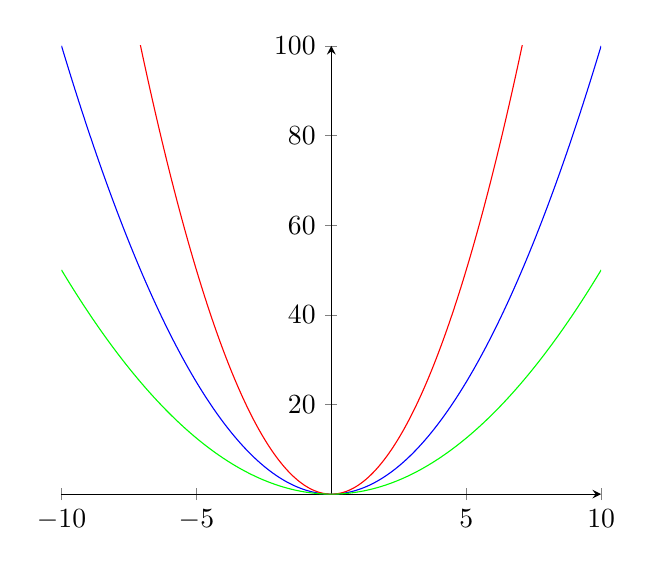
\begin{tikzpicture}[scale = 1.0]
    \begin{axis}[
        domain=-10:10,
        xmin=-10, xmax=10,
        ymin=-0, ymax=100,
        samples=400,
        axis y line=center,
        axis x line=middle,
    ]
    	   \addplot+[mark=none, color=blue] { x*x};
        \addplot+[mark=none, color=red] {2 * x*x};
         \addplot+[mark=none, color=green] {0.5 * x*x};
    \end{axis}
\end{tikzpicture}
\end{center}
\caption{Normalparabel (blau), gestreckte (rot) und gestauchte Normalparabel (gr"un).}
\end{figure}

\subsubsection{Die Scheitelform}
Durch Kombination von Stauchung/Streckung und Verschiebung erh"alt man die so genannte Scheitelform: 
\begin{equation*}
f(x)=a(x-x_s)^2+y_s
\end{equation*}
Mithilfe dieser Funktion lassen sich alle Arten quadratischer Funktionen darstellen. Au"serdem lassen sich die Koordinaten des Scheitels, der Stauchungs- bzw. Streckungsfaktor der Funktion, sowie die Frage, ob sie nach oben oder unten ge"offnet ist, auf einfachste Weise bestimmen.

\subsubsection{Die Normalform einer quadratischen Gleichung}
Multipliziert man die Scheitelform aus, so erh"alt man 
\begin{equation*}
f(x)=a \cdot x^2-2 \cdot a \cdot x_sx+x_s^2+y_s.
\end{equation*}
Ersetzt man nun die konstanten Werte $-2ax_s$ durch $b$ und $x_s^2+y_s$ durch $c$, so erh"alt man die \textbf{Normalform} quadratischer Gleichungen:
\begin{equation*}
f(x)=a \cdot x^2+b \cdot x+c
\end{equation*}

\subsubsection{Die binomischen Formeln}
Die binomischen Formeln sind das Ergebnis des Ausmultiplizierens, hat man sie jedoch im Kopf so spart man viel Zeit.
\begin{enumerate}
\item $(a+b)^2=a^2+2ab+b^2$
\item $(a-b)^2=a^2-2ab+b^2$
\item $(a+b)(a-b)=a^2-b^2$
\end{enumerate}

\subsubsection{Die quadratische Erg"anzung}
Die quadratische Erg"anzung hilft uns bei der Umwandlung der Normalform in die Scheitelform und somit bei der Bestimmung des Scheitels. Wir werden diese an anhand eines Beispiels erkl"aren.

\paragraph{Beispiel:}
Sei 
\begin{equation*}
f(x) = 3x^2 - 6x - 24.
\end{equation*}
Im ersten Schritt klammern wir die Konstante "'$a$"' (hier gleich $3$) aus:
\begin{equation*}
f(x) = 3x^2 - 6x - 24= 3 \cdot (x^2-2x-8).
\end{equation*}
Schaut man sich nun den Term innerhalb der runden Klammern genauer an, so kann man eine gewisse "Ahnlichkeit mit der ersten, bzw. zweiten binomischen Formel feststellen. Deshalb folgt nun auch der wichtigste Schritt, die eigentliche quadratische Erg"anzung. Wir erg"anzen die Formel nun so, dass wir eine der beiden binomischen Formeln anwenden k"onnen. Daf"ur m"ussen wir erste einmal feststellen, was der a- und was der $b$-Wert der binomischen Formeln ist. Die zweite binomische Formel lautet 
\begin{equation*}
(a-b)^2=a^2-2ab+b^2.
\end{equation*}
Vergleichen wir dies mit unserem Term 
\begin{equation*}
x^2-2x-8
\end{equation*}
so sehen wir gleich, dass
\begin{equation*}
a := x \Rightarrow 2ab = 2x \Rightarrow b = 1.
\end{equation*}
Allerdings ist $b^2$ f"ur $b = +1$ nicht $-8$ sondern $1$. Um $f$ nicht zu ver"andern m"ussen wir deshalb eine Korrektur vornehmen:
\begin{equation*}
f(x) = 3 \cdot \left(  \underbrace{(x-1)^2}_{\text{wegen 2. bin. Formel}} + \underbrace{-1^2 - 8}_{\text{da } b^2 = 1 \text{ und nicht } -8 } \right)
\end{equation*}
Hier nochmal die "Ubersicht:
\begin{equation*}
f(x) = 3 \cdot \left(  \underbrace{x^2}_{:=a^2} \underbrace{- 2 \cdot x \cdot 1}_{:= -2ab} \underbrace{+ 1^2}_{:= + b^2} \underbrace{- 1^2 -8}_{:=-\text{Korrektur}} \right)
\end{equation*} 
Nun k"onnen wir noch ein wenig zusammenfassen
\begin{equation*}
f(x) = 3 \cdot ((x-1)^2-1^2-8) = 3((x-1)^2-9) = 3(x-1)^2-27
\end{equation*}
Und voil\`a, schon ist man fertig.

\subsubsection{Berechnung der Nullstellen} \label{sec:quadnullstellen}
Um die Nullstellen von quadratischen Gleichungen zu berechnen, gibt es mehrere M"oglichkeiten.

\paragraph{Zerlegung in Linearfaktoren (auch f"ur Polynome):}
\begin{center}
"'Null multipliziert mit irgendwas ist immer Null"'
\end{center}
Mit der Linearfaktorzerlegung erhalten wir eine Form der Funktion, die uns sagt f"ur welche $x$ ein Faktor Null und somit die gesamte Funktion Null ergibt. Auch dies zeigen wir an einem Beispiel.

\paragraph{Beispiel}
Sei
\begin{equation*}
f(x) = 6x^2 - 24
\end{equation*}
Wir fragen uns f"ur welche $x$ ist $f(x) = 0$.
\begin{equation*}
f(x) = 0 \iff 6x^2 - 24 = 0 \iff x^2 - 4 = 0 \iff^{\text{3. bin. Formel}} (x-2)(x+2) = 0 
\end{equation*}
Die Faktoren der Funktion sind somit $(x-2)$ und $(x+2)$. $(x-2) = 0$ f"ur $x = 2$ und $(x+2) = 0$ f"ur  $x = -2$. Damit sind die Nullstellen:
\begin{equation*}
N_1 = (2, f(2)) = (2, 0) \text{ und } N_2 = (-2, f(-2)) = (-2, 0)
\end{equation*}

\paragraph{Berechnung der Umkehrfunktionen (nicht f"ur quadratischen Funktionen):}
Im Grundlagenteil haben wir den Begriff der Umkehrfunktion kennen gelernt. Angenommen $x_0$ sei eine Nullstelle der Funktion $f(x)$ und angenommen $f(x)$ besitzt eine Umkehrfunktion ($f(x)$ ist bijektiv), dann folgt daraus:
\begin{equation*}
f(x_0) = 0 \iff f^{-1}(0) = x_0
\end{equation*}
Das hei"st wir k"onnten $f^{-1}(x)$ berechnen und dann einfach $0$ einsetzten und erhalten damit die Nullstelle von $f(x)$ nämlich $N = (f^{-1}(0), 0)$.

\paragraph{Beispiele}
\begin{itemize}
\item Sei $f(x) = 3x^2 + 3x + 4$: Die Normalparabel ist nicht bijektiv und da jede quadratische Funktion eine gestauchte und verschobene 'Variante' der Normalparabel ist, sind quadratische Funktionen nicht bijektiv.
\item Sei $f(x) = x - 7 \Rightarrow f^{-1}(y) = y + 7 \Rightarrow N = (f^{-1}(0), 0) = (7, 0)$
\end{itemize}

% Was hier folgt ist unsinnig!
%Wenn wir also rein theoretisch die Funktion umkehren und 0 einsetzen, so m"ussten wir die x-Werte der Nullstellen herausbekommen. Wollen wir jedoch eine quadratische Gleichung umkehren, so sto"sen wir allerdings auf ein kleines Problem... \vspace{0.5 cm}\\
%Schauen wir uns daf"ur mal ein Beispiel an:\\
%$y = $\\
%Zun"achst m"usste man daf"ur sorgen, dass das x nicht mehr in zwei verschiedenen Potenzen auftaucht. Dies geht ganz leicht "uber die quadratische Erg"anzung.\\
%$y = 3(x + 0,5)^2 + 3,25 | -3,25\leftrightarrow$\\
%$3(x+0,5)^2 = y-3,25 | :3 \leftrightarrow$\\
%$(x+0,5)^2 = \frac{y-3,25}{3}$\\
%Nun m"ussten wir die Wurzel ziehen. Hier kommt das Problem zum Vorschein.\\
%Die Wurzel einer bestimmten Zahl kann sowohl positiv als auch negativ sein.\\
%Nehmen wir zum Beispiel die Zahl 4: ihre Wurzel ist $\pm 2$.\\
%Da die Regel, dass jedem x-Wert genau ein y-Wert zugeordnet wird, nicht mehr erf"ullt wird, handelt es sich nicht mehr um eine Funktion, sondern um eine Relation.
%Aus diesem Grund gilt auch f"ur unsere Gleichung:\\
%$x+0,5 =\pm \sqrt{\frac{y-3,25}{3}}\leftrightarrow$\\
%$x=0,5 \pm \sqrt{\frac{y-3,25}{3}}$\\
%Nun muss man noch f"ur y  0 einsetzen und gucken was passiert.\\
%In unserem Fall bemerkt man schnell, dass unter der Wurzel ein negativer Wert heraus kommt. Dies darf jedoch nicht sein, da in den reellen Zahlen die Wurzel von negativen Zahlen nicht definiert ist.\\
%Somit hat unsere Funktion keinerlei Nullstellen.

\paragraph{Die Mitternachtsformel:}
Eine weitere M"oglichkeit, die Nullstellen einer quadratischen Funktion zu berechnen, w"are durch Verwendung der so genannten "'Mitternachtsformel"':
\begin{equation*}
0 = ax^2 + bx + c \Rightarrow x_{1,2} := \frac{-b \pm \sqrt{b^2 - 4ac}}{2a}
\end{equation*}
Falls jedoch 
\begin{equation*}
b^2 - 4ac < 0
\end{equation*}
existiert \textbf{keine Nullstelle}, da wir in den reellen Zahlen keine negative Wurzel kennen und falls
\begin{equation*}
b^2 - 4ac = 0
\end{equation*}
handelt es sich um eine sog. \textbf{doppelte Nullstelle}. Ansonsten handelt es sich um \textbf{zwei Nullstellen}. Dabei nennen wir $b^2 - 4ac$ die Diskriminante.
%Wie man sieht, ist es sehr umst"andlich, jedes Mal die Umkehrrelation zu berechnen und in diese dann f"ur y den Wert 0 einzusetzen... Aus diesem Grund wurden allgemeine Formeln zur Berechnung der Nullstellen quadratischer Gleichungen hergeleitet:\\
%Zun"achst hat man die allgemeine Formel $y = ax^2 + bx +c$ gegeben.\\
%Diese wird "'gleich Null"' gesetzt:\\
%$0 = ax^2 + bx + c$\\
Wie entsteht diese Formel?
\begin{equation*}
 ax^2 + bx + c 
\end{equation*}
Wird auf die Scheitelform gebracht
\begin{equation*}
 ax^2 + bx + c  = (x + \frac{b}{2a})^2 - \frac{b^2-4ac}{4a^2}
\end{equation*}
und gleich Null gesetzt
\begin{equation*}
(x + \frac{b}{2a})^2 - \frac{b^2-4ac}{4a^2} = 0 \iff x = \frac{-b \pm \sqrt{b^2 - 4ac}}{2a}
\end{equation*}
Den Beinamen "'Mitternachtsformel"' verdankt sie ihrer Wichtigkeit. Sie wird n"amlich tats"achlich so oft gebraucht, dass man sie auch noch auswendig aufsagen k"onnen sollte, wenn man um Mitternacht geweckt wird! (Auch wenn von euch vermutlich niemand bereits um Mitternacht schl"aft $\ldots$)
Die Mitternachtsformel hat noch einen weiteren Vorteil. Mithilfe der Diskriminante (dem Term, der bei der Mitternachtsformel unter der Wurzel steht) l"asst sich auch auf leichteste Weise feststellen, ob die Funktion Nullstellen besitzt und wenn ja, wie viele.

\paragraph{Raten der Nullstellen (nicht nur f"ur quadratischen Funktionen):}
Ist man erfahren genug und die Funktion einfach genug, so kann man h"aufig die Nullstelle auch einfach erraten. Dann muss man noch einen Beweis erbringen, dass es sich wirklich um einen Nullstelle handelt. Hierf"ur setzten wir einfach das geratene $x_0$ in $f(x)$ ein und "uberpr"ufen ob 
\begin{equation*}
f(x_0) \stackrel{?}{=} 0
\end{equation*}

%\begin{description}
%\item[Zwei Nullstellen] Die Funktion besitzt zwei Nullstellen, wenn der Wert der Diskriminante gr"o"ser 0 ist.
%\item[Eine Nullstelle] Die Funktion besitzt nur eine (doppelte) Nullstelle, wenn die Diskriminante 0 ergibt.
%\item[Keine Nullstelle] Die Funktion hat keinerlei Nullstellen, wenn f"ur die Diskriminante ein Wert kleiner 0 heraus kommt.
%\end{description}

\subsection{"Ubungen zu quadratischen Funktionen}

\begin{enumerate}
\item Berechne die Scheitelpunkte folgender Gleichungen
\begin{itemize}
\item $f(x) = 3x^2 - 3x + 6$
\item $f(x) = x^2 - 8x - 4$
\item $f(x) = x^2 + 4x + 1$
\item $f(x) = -4x^2 + 16x - 1$
\end{itemize}
\item Berechne die Nullstellen der oberen Gleichungen
\end{enumerate}

\subsection{Polynome}
\subsubsection{Was ist ein Polynom}
Bei Funktionen der Form $f(x) = a_n x^b + a_{n-1} x^{b-1} + a_{n-2} x^{b-2} + ... a_0$ handelt es sich um so genannte Polynome.\\

\subsubsection{Nullstellenberechnung mithilfe der Polynomdivision}
Im Folgenden werde ich nun anhand des Beispiels $f(x) = 6x^3 - 12x^2 - 6x + 12$ die Nullstellenberechnung mithilfe der Polynomdivision erl"autern.\\
\begin{enumerate}
\item Zun"achst wird die Funktion gleich Null gesetzt.\\
$6x^3 - 12x^2 - 6x + 12 = 0$
\item Anschlie"send kann man die ganze Funktion einmal durch den Koeffizienten vor dem x mit der h"ochsten Potenz teilen.\\
In unserem Fall also durch den Wert 6.\\
$ x^3 -2x^2 - x + 2 = 0 $
\item Nun muss man, so komisch es auch klingt, zun"achst einmal eine Nullstelle "'erraten"'.\\
Da es aber sehr viele Zahlen gibt, w"urde dies ohne einen kleinen Trick sehr schwer werden.\\
Besitzt ein Polynom lediglich ganzzahlige Koeffizienten, so sind die x-Werte der Nullstellen ganzzahlige Teiler von $a_0$.\\
Unser Beispiel kann also nur Nullstellen bei x-Werten von -1,1,-2,2,-3,3,-6 und 6 besitzen.\\
Nun kann man systematisch alle m"oglichen Kandidaten abarbeiten.\\
Testen mit x = -1:\\
$(-1)^3 - 2(-1)^2 - (-1) + 2 = 0$\\
Gl"ucklicherweise haben wir schon beim ersten Versuch eine Nullstelle entdeckt.\\
\item Nun werden wir uns die Eigenschaft des Faktorisierens zu Nutze machen, dass jedes Polynom in Faktoren $(x-x_{Nullstelle})$ zerlegt werden kann.\\
Wir werden nun n"amlich eine schriftliche Division des Polynoms durch (x-(-1)) durchf"uhren.\vspace{0.5 cm}\\
$ (x^3 - 2x^2 - x + 2):(x+1)= x^2 - 3x + 2$\\
$ \underline{-x^3 - x^2} $\\
$ \hspace{0.75 cm} -3x^2 - x $\\
$ \hspace{0.75 cm} \underline{+3x^2 + 3x} $\\
$ \hspace{1.75 cm} +2x + 2$\\
$ \hspace{1.75 cm} \underline{-2x - 2}$\\
$ \hspace{3 cm} 0$
\item Jetzt beginnt der Vorgang mit der neuen Funktion ($g(x) = x^2 - 3x + 2$), welche einen Grad weniger hat von Neuem. In unserem Fall jedoch, da wir nun eine quadratische Funktion haben, k"onnen wir die Mitternachtsformel zur L"osung heranziehen.\\
Die drei Nullstellen unserer Beispielfunktion lauten:\\
$x_0 = -1; x_1 = 1; x_2 = 2$\\
Die Funktion l"asst sich also auch wie folgt schreiben:\\
$f(x)=(x+1)(x-1)(x-2)$
\end{enumerate}

\subsection{"Ubungen zu Polynomen}
Berechne die Nullstellen folgender Gleichungen
\begin{itemize}
\item $f(x) = x^4 - 2x^2 + 1$
\item $f(x) = 3x^3 + 12x^2 + 3x - 18$
\end{itemize}

\subsubsection{Rechnen mit Exponenten}
Wie ihr vielleicht schon bemerkt habt, gibt es bei den \textcolor{red}{geometrischen Folgen} eine neue mathematische Schreibweise ($q^n$). Die Konstante $q$ wird hierbei als \textcolor{red}{Basis} bezeichnet, während $n$ \textcolor{red}{Exponent} genannt wird. Hierbei gilt:
\begin{itemize}
\item $q^0 = 1$
\item $q^1 = q$
\item $q^2 = q \cdot q$
\item $q^3 = q \cdot q \cdot q$
\item $q^4 = q \cdot q \cdot q \cdot q$
\item $\ldots$
\end{itemize}

\paragraph{Rechengesetze für Exponenten}
\begin{enumerate}
\item $((b)^n)^m = b^{n \cdot m}$
\item $b^n \cdot b^m = b^{n+m}$
\item $\frac{b^n}{b^m} = b^{n-m}$
\end{enumerate}

\paragraph{Rechengesetze für Wurzeln}
\begin{enumerate}
\item $\sqrt[m]{a} = a^{\frac{1}{m}}$
\item $\sqrt[m]{a} \cdot \sqrt[m]{b} = \sqrt[m]{a \cdot b}$
\item $\frac{\sqrt[m]{a}}{\sqrt[m]{b}} = \sqrt[m]{\frac{a}{b}}$
\item $\sqrt[m]{b^n} = b^{\frac{n}{m}}$
\end{enumerate}

\subsection{Trigonometrische Funktionen}
\subsubsection{Die Winkelfunktionen rechtwinkliger Dreiecke}
Grundlegend gibt es drei Winkelfunktionen, welche auf rechtwinklige Dreiecke angewandt werden k"onnen:
\begin{itemize}
\item Sinus $\sin : \mathbb{R} \to \mathbb{R}, \mathbb{W} = \left[-2\pi;+2\pi \right]$
\item Kosinus $\cos : \mathbb{R} \to \mathbb{R}, \mathbb{W} = \left[ -2\pi;+2 \pi \right]$
\item Tangens $\tan : \left( \mathbb{R} \setminus \left\{ k \pi + \frac{\pi}{2}, k \in \mathbb{Z} \right\} \right) \to \mathbb{R}, \mathbb{W} = \mathbb{R}$
\end{itemize}
Der Tangens ist f"ur die Nullstellen des Kosinus nicht definiert denn
\begin{equation*}
\tan(x) := \frac{\sin(x)}{\cos(x)}
\end{equation*}
Die drei Seiten des Dreiecks werden als Hypotenuse (l"angste Seite des Dreiecks, -gegen"uber des rechten Winkels-), Ankathete (kurze Seite, welche am Winkel $\alpha$ anliegt), und Gegenkathete (Seite gegen"uber des Winkels $\alpha$) bezeichnet.
\begin{minipage}{0.45\textwidth}
\hfill
\begin{enumerate}
\item $\sin(\alpha)=\frac{\text{Gegekathete}}{\text{Hypotenuse}}$
\item $\cos(\alpha)=\frac{\text{Ankathete}}{\text{Hypotenuse}}$
\item $\tan(\alpha)=\frac{\sin(\alpha)}{\cos(\alpha)}= \frac{\text{Gegenkathete}}{\text{Ankathete}}$
\end{enumerate}
\end{minipage}
\begin{minipage}{0.45\textwidth}
\includegraphics[width=1.0\textwidth]{pictures/TrigonDreieck}
\end{minipage}

\subsubsection{Der Einheitskreis}
Am besten sieht man die Eigenschaften der Winkelfunktionen bei der Betrachtung des \textcolor{red}{Einheitskreises}. Der Einheitskreis ist an sich nichts anderes als ein Kreis, mit Radius $r$ = 1 LE und Kreismittelpunkt im Ursprung. Dabei ist die $x$-Koordinate des Punktes, am Ende der Hypotenuse des eingezeichneten Dreiecks, der Kosinuswert des Winkels Alpha und die $y$-Koordinate der Sinuswert. Der Tangens ist die Steigung der Hypotenuse. Der Zusammenhang zwischen Einheitskreis und den Funktionen ist in Abb. \ref{fig:circ} zu sehen.

\begin{figure}[h!]

\begin{tikzpicture}
% Axis
\draw[thick,-stealth,black] (-3,0)--(4,0) coordinate (A) node[below] {$x$}; % x axis
\draw[thick,-stealth,black] (0,-3)--(0,3) node[left] {$y$}; % y axis
\draw[black,thin] (0,0) circle (2.5cm);
\node[black,below] at (2.7,0) {1};
\node[black,above] at (0.2,-3.2) {1};

\draw[ultra thick,orange] (0,0) -- (\theangle:2.5cm |- 0,0) node[midway,above] {$\cos(\alpha)$}; % UpOn y axis

\draw (1,0) arc (0:\theangle:1) node at ($(\theangle/2:0.7)$) {$\alpha$};
\draw[dashed, cyan] (\theangle:2.5cm) -- (\theangle:2.5cm |- 0,0) node[sloped, rotate=180, yshift=8pt, midway] {$\sin(\alpha)$}; % vertical line
\draw[ultra thick,red,rotate=\theangle] (0,0) -- (2.5,0) coordinate (B); 

\draw[dashed,red] (0,0) -- (-2.5,-2.097);

\draw[ultra thick, blue] (-2.5,0) -- (-2.5,-2.097) node[sloped, midway,below] {$\tan(\alpha)$};;

\foreach \x in {0,30,...,360} {\filldraw[black] (\x:2.5cm) circle(1pt);};
\foreach \x/\xtext in {
        30/\frac{\pi}{6},
        60/\frac{\pi}{3},
        120/\frac{2\pi}{3},
        150/\frac{5\pi}{6},
        210/\frac{7\pi}{6},
        240/\frac{4\pi}{3},
        300/\frac{5\pi}{3},
        330/\frac{11\pi}{6}
        }
    \draw (\x:2.8cm) node {\tiny $\xtext$};
 \foreach \x/\xtext in {
        90/\frac{\pi}{2}}
        \draw (\x:2.7cm) node[xshift=4pt] {\tiny $\xtext$};    
 \foreach \x/\xtext in {
        270/\frac{3\pi}{2}}
        \draw (\x:2.7cm) node[xshift=-5pt] {\tiny $\xtext$};  
 \foreach \x/\xtext in {
        180/\pi,
        360/2\pi}
        \draw (\x:2.7cm) node[yshift=4pt] {\tiny $\xtext$};             

\begin{scope}
\begin{axis}[
    thick,
    y=2.5cm,
    axis lines=center,
    xmin=0, xmax=360,
    ymin=-1, ymax=1,
    anchor=origin, at=(A),
    xshift=3ex,
    enlarge y limits,
    enlarge x limits=upper,
    samples=90,
    xtick={0,30,...,360},
xticklabels={0,
    $\frac{\pi}{6}$,
    $\frac{\pi}{3}$,
    $\frac{\pi}{2}$,        
    $\frac{2\pi}{3}$,
    $\frac{5\pi}{6}$,
    $\pi$,
    $\frac{7\pi}{6}$,
    $\frac{4\pi}{3}$,
    $\frac{3\pi}{2}$,        
    $\frac{5\pi}{3}$,
    $\frac{11\pi}{6}$,
    $2\pi$
    },
    tick label style={font=\tiny},
    ]
    \addplot[domain=0:\theangle,ultra thick, no markers,cyan] {sin(x)} coordinate (C);
    \addplot[domain=\theangle-1:\theangle,ultra thick, no markers,cyan] {sin(x)-sin(x)} coordinate (K);

\end{axis}
\draw [dashed,red, thick] (B) -- (C);
\draw [dashed,cyan, thick] (C) -- (K);
\end{scope}
\tkzDrawPoints(B);
\end{tikzpicture}
\caption{Einheitskreis (links) und die Sinusfunktion (rechts).}
\label{fig:circ}
\end{figure}

\subsubsection{Winkelma"s und Bogenma"s}
Bisher haben wir immer mit Winkelma"sen gerechnet, wie zum Beispiel $\alpha = 45^\circ$. Neben dieser M"oglichkeit, Winkel auszudr"ucken, gibt es auch noch das Bogenma"s $b = 2\pi \ rad$. Das Bogenma"s ist die L"ange des Kreisbogens mit dem Radius $r = 1$ unter einem bestimmten Winkel. Die Umrechnung ist einfach
\begin{equation*}
rad(\alpha) = 2\pi \frac{\alpha}{360} rad \text{ f"ur } \alpha \in \left[ 0^\circ;360^\circ \right] \quad rad^{-1}(b) = 360 \cdot {\frac{b}{2\pi}}^\circ \text{ f"ur } b \in \left[0;2\pi\right]
\end{equation*}
Wie ein Winkelwert mit $^\circ$ gekennzeichnet wird, so kennzeichnet man das Bogenma"s mit dem W"ortchen "'$rad$"'. An den meisten "'h"oheren"' Schulen wird das Bogenma"s bevorzugt.

\begin{figure}[h!]
\includegraphics[width = 13 cm, height = 5 cm]{pictures/Winkelfunktionen}
\caption{Funktionsgraphen von Sinus, Kosinus und Tangens}
\end{figure}

\subsubsection{Nullstellen, Asymptoten und Symmetrie}
Alle Winkelfunktionen sind periodisch. Deshalb treten auch ihre Nullstellen in gleichbleibenden Abst"anden auf.
\begin{itemize}
\item Sinusfunktion:
\begin{equation*}
 \sin(x) = 0 \iff x \in \left\{ k \pi, k \in \mathbb{Z} \right\},
\end{equation*}
was sich mit den Nullstellen des Tangens deckt.
\item Kosinusfunktion: 
\begin{equation*}
 \cos(x) = 0 \iff x \in \left\{ k \pi + \frac{\pi}{2}, k \in \mathbb{Z} \right\},
\end{equation*}
was sich mit den Definitionsl"ucken des Tangens deckt.
\end{itemize}
Des Weiteren besitzt die Tangensfunktion eine periodisch auftretende senkrechte Asymptote an den Nullstellen des Kosinus.
Betrachtet man die Graphen im Hinblick auf ihre Symmetrie bez"uglich des Koordinatensystems, stellt man fest, dass die Sinus- und Tangesnsfunktion \textbf{punktsymmetrisch} zum Ursprung (ungerade) und die Kosinusfunktion achsensymmetriesch zur $y$-Achse (gerade) ist.

\psection{Differentiation}
Beim Ableiten m"ochten wir etwas "uber die Ver"anderung einer Funktion erfahren. Angenommen ein Auto startet an einem Punkt und die Funktion $s(t)$ gibt an wie viele Meter das Auto zum Zeitpunkt $t$ zur"uckgelegt hat. Wir fragen uns nun wie schnell das Auto nach 10 Sekunden f"ahrt. Wie k"onnen wir dies herausfinden? Wir k"onnen das absch"atzen indem wir 
\begin{equation*}
\bar{v} = \frac{\text{Strecke}}{\text{Zeit}} \approx \frac{s(11) - s(9)}{11 - 9} = \frac{\Delta s}{\Delta t} = \frac{s(11) - s(9)}{2}
\end{equation*}
Aber ist $\bar{v} \stackrel{?}{=} v(10)$? Nein $\bar{v}$ ist nur die durchschnittliche Geschwindigkeit zwischen $s(9)$ und $s(11)$. Wenn wir die Geschwindigkeit genauer bestimmen m"ochten, m"ussen wir den Abstand/die \textit{Umgebung} von/um $10$ kleiner w"ahlen, $0$ darf er jedoch nicht werden, denn wir d"urfen nicht durch Null teilen. Hilfe gibt uns der Grenzwert:
\begin{equation*}
v(10) = \lim\limits_{h \to 0} \frac{s(10+h) - s(10)}{h}
\end{equation*}
Der Grenzwert muss nat"urlich existieren! Nehmen wir einmal an das Auto beschleunigt und $s(t) = 2 t^2$.
\begin{align*}
v(10) &= \lim\limits_{h \to 0} \frac{s(10+h) - s(10)}{h} = \lim\limits_{h \to 0} \frac{2 (10+h)^2 - 2 (10)^2}{h}\\
&= \lim\limits_{h \to 0} \frac{40h + 2h^2}{h} = \lim\limits_{h \to 0}(40 + 2h) \to 40
\end{align*}

\subsection{Ableiten von Funktionen}
Die Ableitung der Funktion $f$ an der Stelle $x_0$, geschrieben $f'(x_0)$ beschreibt das Verhalten der Funktion in der \textit{Umgebung} an der Stelle $x_0$. Sie ist auch die Steigung der Funktion an dem Punkt $x_0$. Die Tangente an $x_0$ hat die Steigung $f'(x_0)$. Eine Tangente ist eine Gerade, die den Graphen in nur einem einzigen Punkt ber"uhrt. Um die Tangentensteigung zu erhalten, betrachtet man zun"achst die Steigung einer Sekante und n"ahert den zweiten Punkt dem ersten immer weiter an.
\begin{definition}[Differenzierbarkeit in $x_0$]
Eine Funktion hei"st differenzierbar an der Stelle $x_0$ wenn der Grenzwert
\begin{equation*}
 \lim\limits_{x \to x_0} \frac{f(x)-f(x_0)}{x-x_0} = \lim\limits_{h \to 0}  \frac{f(x_0 + h)-f(x_0)}{h} , \text{ mit } h = x - x_0
\end{equation*}
existiert. Dieser Grenzwert wird Ableitung nach $x$ an der Stelle $x_0$ genannt und wird als $f'(x_0)$ oder $\frac{df}{dx}(x_0)$ notiert.
\end{definition}
Ein Grenzwert $a$ an der Stelle $x_0$ der Funktion $f$ existiert wenn der linke Grenzwert gleich dem rechten Grenzwert gleich dem Funktionswert gleich $a$ ist, also
\begin{equation*}
 \lim\limits_{x \to x_0^+} \frac{f(x)-f(x_0)}{x-x_0} =  \lim\limits_{x \to x_0^-} \frac{f(x)-f(x_0)}{x-x_0} = f(x_0) = a
\end{equation*}

\begin{definition}[Differenzierbarkeit]
Eine Funktion hei"st differenzierbar, wenn sie an jeder Stelle $x_0 \in \mathbb{D}$ differenzierbar ist.
\end{definition}

\paragraph{Anmerkung:} Eine differenzierbare Funktion ist stetig und eine in $x_0$ differenzierbare Funktion ist stetig in $x_0$. Die Umkehrung gilt nicht!

\subsubsection{Die erste Ableitung}
F"ur die gew"ohnlichen differenzierbaren Funktionen gibt es die uns bekannten Ableitungsregeln. Um eine Funktion abzuleiten multipliziert man bei Polynomen jeweils die Exponenten mit den dazugeh"origen Koeffizienten ihrer Basis und subtrahiert den Exponenten dabei um 1. Konstanten fallen dabei weg.
\begin{equation*}
f(x) = a_1 \cdot (x-a_2)^{a_3} + a_4 \Rightarrow f'(x) = a_1 \cdot (x - a_2)^{a_3-1} \cdot a_3 \text{ mit } a_1,a_2,a_3 \text{ konstant.}
\end{equation*}

\paragraph{Beispiel:}
\begin{equation*}
f(x)=2x^2 \Rightarrow f'(x)= 2 \cdot 2x^{2-1}=4x
\end{equation*}

\subsection{Besondere Ableitungen}
F"ur Logarithmus- und $e$-Funktionen sowie die Winkelfunktionen gelten besondere Ableitungsgesetze:
\begin{itemize}
\item $\sin'(x) = \cos(x)$
\item $\cos'(x) = - \sin(x)$
\item $\tan'(x) = \frac{1}{\cos^2(x)}$
\item $\ln'(x) = \frac{1}{x}$
\item $(e^x)' = e^x$
\end{itemize}

\subsection{Ableitungsregeln}
Wie "uberall in der Mathematik gibt es auch f"ur das Ableiten, insbesondere bei komplizierteren Funktionstermen, bestimmte Regeln im Hinblick auf ihre richtige Ableitung.

\subsubsection{Produktregel}
\begin{equation*}
f(x) = h(x) \cdot g(x) \Rightarrow f'(x)=h'(x) \cdot g(x)+h(x) \cdot g'(x)
\end{equation*}

\paragraph{Beispiel:}
\begin{equation*}
f(x)=2x^3 \cdot \sin(x)\Rightarrow f'(x)=6x^2 \cdot \sin(x)+2x^3 \cdot \cos(x)
\end{equation*}

\subsubsection{Quotientenregel}
\begin{equation*}
f(x)=\frac{h(x)}{g(x)} \Rightarrow f'(x)=\frac{h'(x) \cdot g(x)-h(x) \cdot g'(x)}{(g(x))^2}
\end{equation*}
Diese Regel kann auf die Produktregel zur"uckgef"uhrt werden man bemerke $\frac{h(x)}{g(x)} = h(x) \cdot g(x)^{-1}$

\paragraph{Beispiel:}
\begin{equation*}
f(x)=\frac{2x^3}{2x^2+4} \Rightarrow f'(x)=\frac{6x^2 \cdot (2x^2+4)-2x^3 \cdot 4x}{(2^2+4)^2}
\end{equation*}

\subsubsection{Kettenregel}
F"ur ineinander geschachtelte (verkettete) Funktionen gilt die sogenannte Kettenregel. Diese ist besonders n"utzlich und wird oft mehrmals hintereinander angewendet! Dabei wird die Funktion ganz normal abgeleitet und die innere Funktion \textcolor{red}{nachdifferenziert}.
\begin{equation*}
f(x)=f(g(x))\Rightarrow f'(g(x))=f'(g(x))\textcolor{red}{g'(x)}
\end{equation*}

\paragraph{Beispiel:}
\begin{equation*}
f(g(x))=x^{(x^2+4)}\Rightarrow f'(g(x))=(x^2+4)*x^{(x^2+4-1)}\textcolor{red}{ \cdot 2x}
\end{equation*}

\subsection{"Ubungen}
\begin{enumerate}
\item Bilde die Ableitungen folgender Terme
\begin{itemize}
\item $f(x)=12x^3 - 3x^2 + x + 12$
\item $f(x)= 6 \sin^2(x) + \cos(x) $
\item $f(x)= \frac{x^2-x}{x^2+x}$
\item $f(x)= \frac{3x}{12x^2 - 4x + 2} \cdot \sin^2(x) - 3 \cos(x) + 1$
\end{itemize}
Welche dieser Funktionen sind nicht differenzierbar?
\begin{itemize}
\item $f(x)=\lbrace^{3x; f"ur x < 3}_{2x; f"ur x>3}$
\item $f(x)=|x|$
\item $f(x)= \frac{x^3}{\sin(x)}$
\item $f(x)= 0$
\end{itemize}
\end{enumerate}

\subsection{Kurvendiskussion}
Definition: Bei einer Kurvendiskussion wird der Graph einer Funktion im Hinblick auf seine Eigenschaften, wie seinen \textcolor{red}{Definitionsbereich}, \textcolor{red}{Grenzwerte}, \textcolor{red}{Asymptoten}, \textcolor{red}{Schnittpunkte mit den Koordinatenachsen}, \textcolor{red}{Symmetrie}, \textcolor{red}{Extrem- und Terrassenpunkte}, \textcolor{red}{Monotonie} und seinem \textcolor{red}{Kr"ummungsverhalten}, anhand des Funktionsterms untersucht.
\subsubsection{Definitonsbereich}
Zunächst beschreibt man, in welchem Bereich die Funktion definiert ist, indem man seine Definitions- und Wertemenge bestimmt.
\subsubsection{Schnittpunkte mit den Koordinatenachsen}
Interessant k"onnen auch die Schnittpunkte des Graphen mit den Koordinatenachsen sein, v.a. wenn man den Graphen skizzieren m"ochte.\\
\paragraph{Schnittpunkt mit der y-Achse}\hspace{2 cm}\\
Diesen erh"alt man, wenn man f"ur x den Wert 0 einsetzt.
\paragraph{Nullstellen}\hspace{2 cm}\\
Als n"achstes untersucht man die Funktion auf Nullstellen. Diese erh"alt man, indem man den Funktionsterm gleich Null setzt und nach x aufl"ost.\\
Merke: Ein Polynom hat h"ochstens so viele Nullstellen wie der h"ochste Exponent der Funktion, dabei erh"alt man zum Teil auch mehrfache Nullstellen, wie beispielsweise bei $x^3$. Diese Funktion hat ein dreifache Nullstelle an der Stelle x=0.
\subsubsection{Grenzwerte}
Nun betrachtet man das Verhalten des Graphen im Unendlichen. Dieses gibt man mit Hilfe des Limes an. Dabei ist interessant, ob sich der Graph einem bestimmten Wert ann"ahert oder ob er ins Unendliche steigt oder f"allt.
\subsubsection{Asymptoten}
 Asymptoten k"onnen Geraden aber auch andere Funktionen sein, an die sich der Graph der zu untersuchenden Funktion beliebig nah ann"ahert, ohne sie jemals zu ber"uhren.\\
 Asymptoten findet man vor allem bei gebrochen rationalen Funktionen. Dort, wo der Nenner den Wert 0 erreichen w"urde (an dieser Stelle ist die Funktion nicht definiert $=>$ Grenzwertbildung), befindet sich eine senkrechte Asymptote. Diese Stelle nennt man Polstelle. Es kann aber auch sein, dass es sich dort um ein Loch handelt, dies ist dann der Fall, wenn die Polstelle gleichsam eine Nullstelle der Funktion ist.\\
 Beispiel: $\frac{2x}{4x-1}$ Der Nenner wird 0 bei x=0.25, es handelt sich dabei um keine Nullstelle, somit befindet sich an der Stelle x=0,25 eine senkrechte Asymptote.\\
 Um den Graphen auf waagrechte oder andere Asymptoten zu untersuchen, schaut man sich die Exponenten der Variablen an.\\
 Die folgenden Ausf"uhrungen beziehen sich rein auf die h"ochsten Exponenten der Variablen im Z"ahler und Nenner.
 \subsubsection{Symmetrie}
 Hier untersuchen wir die Symmetrie die Graphen zum Koordinatensystem.\\
 Wir unterscheiden dabei Punktsymmetrie zum Koordinatenursprung und Achsensymmetrie zur y-Achse.\\
 Dabei untersucht man den Funktionsterm auf folgende Weise:
 \begin{itemize}
 \item Achsensymmetrie (y-Achse), wenn $f(x)=f(-x)$
 \item Punktsymmetrie (Ursprung), wenn $f(-x)=-f(x)$
 \end{itemize}
 \subsubsection{Extrem- und Terrassenpunkte}
  F"ur die Untersuchung des Funktionsgraphen ben"otigt man zun"achst die \textcolor{red}{erste Ableitung} des Funktionsterms. Bei einem Extrempunkt findet ein Vorzeichenwechsel der Steigung statt, d.h. die Ableitung ergibt in diesem Punkt 0. Bei einem Terrassenpunkt ist die Ableitung ebenfalls 0. Folglich m"ussen wir, um diese Punkte zu erhalten, die erste Ableitung gleich Null setzen.\\
  Somit ist die Nullstelle der ersten Ableitung entweder ein Extrem- oder Terrassenpunkt.\\
  Ob es sich um einen Extrempunkt oder einen Terrassenpunkt handelt, erfahren wir mit Hilfe der zweiten Ableitung.
  Wenn die Werte der zweiten Ableitung ungleich 0 sind, handelt es sich um einen Extrempunkt.\\
  Ist die zweite Ableitung an dieser Stelle jedoch 0, so wissen wir weiterhin nicht, ob es sich um einen Extrem- oder Terrassenpunkt handelt.\\
  Dabei gilt: 
  \begin{itemize}
  \item ist die zweite Ableitung negativ, handelt es sich um ein lokales Maximum
  \item ist die zweite Ableitung positiv, handelt es sich um ein lokales Minimum
  \end{itemize}
  Kurz: ein lokales Maximum oder Minimum besteht immer dann, wenn die erste Ableitung an ihrer Nullstelle einen Vorzeichenwechsel hat. Andernfalls handelt es sich um einen Terrassenpunkt.
 \subsubsection{Monotonie}
  Nachdem wir die Funktion hinreichend auf Extrem- und Terrassenpunkte untersucht haben, kann man ihre Monotonie analysieren. Diese gibt man "ublicherweise in Intervallen an, deren Grenzen die Ränder und die Extremstellen bilden.
  \subsubsection{Kr"ummung}
 Um das Kr"ummungsverhalten einer Funktion zu untersuchen, ben"otigt man die zweite Ableitung des Funktionsterms.\\
 Es gilt: $f''(x)<0 \Rightarrow \textcolor{red}{rechtsgekr"ummt}$\\
 \hspace{1.4 cm}$f''(x)>0 \Rightarrow \textcolor{red}{linksgekr"ummt}$\\
 Die Stelle, an welcher der Graph seine Kr"ummung "andert, bezeichnet man als Wendestelle.\\
 Diese ist gleich der Nullstelle der zweiten Ableitung des Funktionsterms, d.h. die zweite Ableitung gleich 0 setzten und den zugeh"origen x-Wert berechnen.\vspace{0.5 cm}\\
 Das sind die wesentlichen Schritte einer Kurvendiskussion. Die Reihenfolge der Bearbeitung kann dabei nat"urlich variiert werden. Punkte, an denen sich die Richtung der Kr"ummung von rechts nach links, bzw. von links nach rechts "andert, nennt man Wendepunkte.
 \subsection{"Ubungen}
 \begin{enumerate}
 \item Diskutiere die Kurven folgender Funktionen
 \begin{itemize}
 \item $f(x)=x^4$
 \item $f(x)=sin(x)$
 \item $f(x)=3x^2 + 12x - 4$
 \item $f(x)=\frac{4x^3 + x^2 - x}{x+1}$
 \item $f(x)=\frac{tan^2(x)}{sin^2(x)}$
 \end{itemize}
 \item Untersuche folgende Funktionen auf ihre Nullstellen, Extrempunkte und Kr"ummung.
 \begin{itemize}
 \item $f(x)=(x-4)^2-3$
 \item $f(x)=(x-2)(x+5)(x-4)$
 \item $f(x)=\frac{1}{x}$
 \end{itemize}
 \end{enumerate}
 
 

\psection{Kurvendiskussion}
Die Kurvendiskussion ist die Analyse einer Funktion im Hinblick auf ihre Eigenschaften, wie ihren \textcolor{red}{Definitionsbereich}, \textcolor{red}{Grenzwerte}, \textcolor{red}{Asymptoten}, \textcolor{red}{Schnittpunkte mit den Koordinatenachsen}, \textcolor{red}{Symmetrie}, \textcolor{red}{Extrem- und Terrassenpunkte}, \textcolor{red}{Monotonie} und ihrem \textcolor{red}{Kr"ummungsverhalten}. Die Reihenfolge spielt durchaus eine Reihenfolge. Es macht z.B. keinen Sinn den Wertebereich vor dem Definitionsbereich zu bestimmen, da der Wertebereich direkt vom Definitionsbereich abh"angt.

\subsection{Definitons- und Wertebereich}
Der Definitionsbereich ist die Menge aus der $x$ stammt f"ur, welche die Funktion definiert ist. Wir m"ochten meist den maximalen Definitionsbereich bestimmen, den Bereich also m"oglichst wenig einschr"anken. So ist $f(x) = \sqrt{x}$ f"ur negative reelle Zahlen nicht definiert. Damit w"are ein m"oglicher Definitionsbereich 
\begin{equation*}
\mathbb{D} := \mathbb{R}^{\geq 0} = \left\{x \in \mathbb{R} | x \geq 0 \right\}
\end{equation*}
Ein ebenfalls g"ultiger Definitionsbereich w"are $\left[10;15\right]$. Solche Einschr"ankungen machen Sinn wenn uns nur dieser Bereich der Funktion interessiert. In der Kurvendiskussion werden Sie aber immer nach dem maximalen Definitionsbereich gefragt. Oftmals k"onnen wir eine Funktion vereinfachen, sobald der Definitionsbereich definiert ist. So kann die Funktion
\begin{equation*}
f_1(x) = \frac{x-1}{x-1}
\end{equation*}
durch $f_2(x) = 1$ mit $\mathbb{D}_{f_2} = \mathbb{R} \setminus \{1\}$ ersetzt werden. Man bedenke $f_1(x) = f_2(x) \ \forall x \in \mathbb{D}_{f_2}$ jedoch gilt $f_2(1) = 1$ und $f_1(1)$ ist nicht definiert. Um den Wertebereich einer Funktion $F$ zu bestimmen, bestimmen wir
\begin{equation*}
\mathbb{W}_f = (\mathbb{D}_f) = \left\{f(x) \ | \ x \in \mathbb{D}_f \right\}
\end{equation*}
hierzu kann es von n"oten sein zuerst die Grenzwerte (Abschnitt \ref{sec:grenzwerte}) zu betrachten.

\subsection{Schnittpunkte mit den Koordinatenachsen}
Interessant k"onnen auch die Schnittpunkte des Graphen mit den Koordinatenachsen sein, v.a. wenn man den Graphen skizzieren m"ochte.

\paragraph{Schnittpunkt mit der y-Achse:} $f(0)$, einfach einsetzten und ausrechnen.

\paragraph{Nullstellen:} $f(x) = 0$ (siehe Abschnitt \ref{sec:nullstellen} und \ref{sec:quadnullstellen}). Merke: Ein Polynom hat h"ochstens so viele Nullstellen wie der h"ochste Exponent der Funktion, dabei erh"alt man zum Teil auch mehrfache Nullstellen, wie beispielsweise bei $x^3$. Diese Funktion hat ein dreifache Nullstelle an der Stelle x=0.

\subsection{Grenzwerte} \label{sec:grenzwerte}
\subsubsection{Polstellen und L"ocher}
Eine Polstelle oder ein Pol, ist eine einpunktige Definitionsl"ucke einer Funktion, wenn die Funktionswerte in jeder Umgebung des Punktes (betragsm"a"sig) beliebig gro"s werden. Der Punkt $x_0 = 1$ der Funktion $f_1$ erf"ullt dies nicht (hier handelt es sich um ein \textbf{Loch}), denn $f_1(x) = 1$ in der Umgebung von $x_0$. Betrachten wir 
\begin{equation*}
f(x) := \frac{1}{x-1}
\end{equation*}
so handelt es sich bei $x_0 = 1$ um einen Pol der Funktion $f$ da
\begin{equation*}
\lim\limits_{x \to 1^+} f(x) = \infty \text{ und } \lim\limits_{x \to 1^-} f(x) = -\infty
\end{equation*}
$1^+$ ist der \textbf{rechter Grenzwert} bei $x=1$ (ann"aherung von rechts) und $1^-$ ist der \textbf{linke Grenzwert} bei $x=1$ (ann"aherung von links). Genau dieses Verhalten, also die Grenzwerte interessieren uns bei den Polstellen.

\subsubsection{Verhalten im Unendlichen}
Nun betrachtet man das Verhalten des Graphen im Unendlichen, also
\begin{equation*}
\lim\limits_{x \to +\infty} f(x) \text{ und } \lim\limits_{x \to -\infty} f(x) 
\end{equation*}
Dieses gibt man mit Hilfe des Limes an. Dabei ist interessant, ob sich der Graph einem bestimmten Wert ann"ahert oder ob er ins Unendliche steigt oder f"allt.

\subsection{Asymptoten}
Sei $f$ eine Funktion, so ist eine Asymptote von $f$ eine Gerade die $f$ im Unendlichen, sowohl in $x$ als auch in $y$ Richtung, ann"ahert. Asymptoten gehen somit direkt mit den Grenzwerten der Funktion $f$ einher. Im Normalfall handelt es sich um eine Gerade. Die Gerade muss keine Funktionsgerade sein! Betrachten wir erneut 
\begin{equation*}
f(x) = \frac{1}{x-1}
\end{equation*}
so ist die Gerade $x=0$ eine Asymptote von $f$. $y=1$ ist die triviale Asymptote.
%Asymptoten k"onnen Geraden aber auch andere Funktionen sein, an die sich der Graph der zu untersuchenden Funktion beliebig nah ann"ahert, ohne sie jemals zu ber"uhren. Asymptoten findet man vor allem bei gebrochen rationalen Funktionen. Dort, wo der Nenner den Wert 0 erreichen w"urde (an dieser Stelle ist die Funktion nicht definiert $=>$ Grenzwertbildung), befindet sich eine senkrechte Asymptote. Diese Stelle nennt man Polstelle. Es kann aber auch sein, dass es sich dort um ein Loch handelt, dies ist dann der Fall, wenn die Polstelle gleichsam eine Nullstelle der Funktion ist. Beispiel: $\frac{2x}{4x-1}$ Der Nenner wird 0 bei x=0.25, es handelt sich dabei um keine Nullstelle, somit befindet sich an der Stelle x=0,25 eine senkrechte Asymptote. Um den Graphen auf waagrechte oder andere Asymptoten zu untersuchen, schaut man sich die Exponenten der Variablen an. Die folgenden Ausf"uhrungen beziehen sich rein auf die h"ochsten Exponenten der Variablen im Z"ahler und Nenner.

 \subsection{Symmetrie}
 Hier untersuchen wir die Symmetrie die Graphen zum Koordinatensystem. Wir unterscheiden dabei \textbf{Punktsymmetrie} zum Koordinatenursprung und \textbf{Achsensymmetrie zur $y$-Achse}:
 \begin{itemize}
 \item Achsensymmetrie ($y$-Achse), wenn $f(x)=f(-x)$
 \item Punktsymmetrie (Ursprung), wenn $f(-x)=-f(x)$
 \end{itemize}
 siehe Abschnitt \ref{sec:symmetrie}

\subsection{Extrem- und Terrassenpunkte}
Angenommen Sie sind mit dem Auto unterwegs und sei $v(t)$ die Geschwindigkeit zum Zeitpunkt $t$. Sie beschleunigen und reduzieren die Beschleunigung auf $0$ zur Zeit $t_0$. Nun gibt es 2 M"oglichkeiten:
\begin{enumerate}
\item Sie bremsen: lokaler- oder globaler Extrempunkt von $v(t)$
\item Sie beschleunigen wieder: Terrassenpunkt bin $v(t)$
\end{enumerate}
Wenn sie bremsen (negative Beschleunigung), ist klar, dass sie zum Zeitpunkt $t_0$ eine lokale oder globale Geschwindigkeit erreicht haben. Beschleunigen sie wieder, war die Beschleunigung gleich Null $v(t)$, steigt dann aber wieder an. Um nun herauszufinden wann sie die maximale Geschwindigkeit erreicht haben, m"ussen wir den Zeitpunkt finden, an dem Sie beginnen zu bremsen. D.h. an dem die Beschleunigung gleich Null und somit die Ableitung von $v(t)$ gleich Null ist. Das gibt uns \textbf{m"ogliche} Punkte, es k"onnte aber sein, dass Sie wieder beschleunigt haben. Falls dies der Fall ist h"atte sich die Beschleunigung in der Umgebung um $t_0$ nicht ge"andert und damit w"are die Ableitung der Beschleunigung also die 2. Ableitung von $v$ an $t_0$ gleich Null. Andernfalls handelt es sich um den ersten Fall, also um einen Extrempunkt. Im Allgemeinen wissen wir:
\begin{equation*}
f'(x_0) = 0 \Rightarrow x_0 \text{ ist ein Extrem- oder Terrassenpunkte}
\end{equation*}
Mit der 2. Ableitung ergibt sich folgendes:
\begin{itemize}
\item $f''(x_0) = 0 \Rightarrow x_0 \text{ ist Terrassenpunkte}$ 
\item $f''(x_0) < 0 \Rightarrow x_0 \text{ ist lokales Maximum }$
\item $f''(x_0) > 0 \Rightarrow x_0 \text{ ist lokales Minimum}$
\end{itemize}
Kurz: ein lokales Maximum oder Minimum besteht immer dann, wenn die erste Ableitung an ihrer Nullstelle einen Vorzeichenwechsel hat. Andernfalls handelt es sich um einen Terrassenpunkt, dies k"onnen wir auch "uberpr"ufen ohne die 2. Ableitung zu berechnen.

 \subsection{Monotonie}
Nachdem wir die Funktion hinreichend auf Extrem- und Terrassenpunkte untersucht haben, kann man ihre Monotonie analysieren. Diese gibt man "ublicherweise in Intervallen an, deren Grenzen die Ränder und die Extremstellen bilden. Um beim obigen Beispiel zu bleiben gibt uns die Monotonie die separierten Bereiche an denen wir Beschleunigt bzw. Abgebremst haben.

\subsection{Kr"ummung}
Um das Kr"ummungsverhalten einer Funktion zu untersuchen, ben"otigt man die zweite Ableitung des Funktionsterms. Es gilt: 
 \begin{itemize}
 \item $f''(x_0)<0 \Rightarrow f \text{ ist an } x_0 \ \textcolor{red}{rechtsgekr"ummt} $
 \item $f''(x_0)>0 \Rightarrow f \text{ ist an } x_0 \ \textcolor{red}{linksgekr"ummt}$
 \end{itemize}
Die Stelle $x_0$, an welcher der Graph seine Kr"ummung "andert, bezeichnet man als Wendepunkt, hier "andert sich die Richtung der Kr"ummung von rechts nach links, bzw. von links nach rechts. Der Wendepunkt ist gleich der Nullstelle der 2. Ableitung des Funktionsterms, d.h. die zweite Ableitung gleich $0$ setzten und den zugeh"origen $x$-Wert berechnen. Das sind die wesentlichen Schritte einer Kurvendiskussion.

 \subsection{"Ubungen}
 \begin{enumerate}
 \item Diskutiere die Kurven folgender Funktionen
 \begin{itemize}
 \item $f(x)=x^4$
 \item $f(x)=\sin(x)$
 \item $f(x)=3x^2 + 12x - 4$
 \item $f(x)=\frac{4x^3 + x^2 - x}{x+1}$
 \item $f(x)=\frac{\tan^2(x)}{\sin^2(x)}$
 \end{itemize}
 \item Untersuche folgende Funktionen auf ihre Nullstellen, Extrempunkte und Kr"ummung.
 \begin{itemize}
 \item $f(x)=(x-4)^2-3$
 \item $f(x)=(x-2)(x+5)(x-4)$
 \item $f(x)=\frac{1}{x}$
 \end{itemize}
 \end{enumerate}
 
 

\psection{Integration (Bonus)}
\subsection{Integration}
Definition (Integral): ein Integral ist die Fl"achenbilanz zwischen einem Funktionsgraphen und der x-Achse.\\
Integrale werden immer in Intervallen berechnet.\\
Dabei unterscheidet man offene Integrale, d.h ein Integral ohne Grenzen und ein geschlossenes Integral, welches lediglich in einem bestimmten Intervall berechnet wird.\\
Schreibweise: $\int f(x)dx\Rightarrow$  offenes Integral\\
\hspace{2.5 cm}$\int\limits_{a}^{b}f(x)dx \Rightarrow$ geschlossenes Integral im Intervall [a;b]\\
Dabei beschreibt das dx am Ende jeweils, nach welcher Variable integriert wird. In der Physik beispielsweise findet man auch h"aufig die Bezeichnung dt.
\subsubsection{Stammfunktionen}
Definition: die Ableitung einer Stammfunktion ergibt den Funktionsterm der urspr�nglichen Funktion.\\
Symbol der Stammfunktion: F(x)     d.h. $F'(x)=f(x)$
\subsubsection{Berechnung von Stammfunktionen}
Die Stammfunktion erh"alt man, indem man die Ableitung r"uckw"arts rechnet. D.h. ich addiere den Exponenten um 1, bilde daraus einen Bruch der Form $\frac{1}{Exponent+1}$ und multipliziere diesen mit dem Faktor vor der Basis.
Mit dieser Methode lassen sich zu fast allen Polynomen Stammfunktionen berechnen. Da es sich um eine Stammfunktion handelt, muss sie am Ende noch mit einer unbekannten Konstanten C addiert werden.
\subsubsection{Hauptsatz der Differential- und Integralrechnung (HDI)}
\textcolor{red}{HDI}:\textcolor{red}{!!!Jede Integralfunktion ist eine Stammfunktion der zu integrierenden Funktion!!!}
\subsubsection{Berechnung von Integralen}
Zun"achst berechnet man sich eine Stammfunktion der Integralfunktion.\\
$\int\limits_{a}^{b} f(x)dx \Rightarrow [F(x)]^b_a$\\
Als n"achstes setzt man die obere Grenze in die Stammfunktion ein und subtrahiert von diesem Wert den Wert der Stammfunktion mit der eingesetzten unteren Grenze.\\
$F(b)-F(a)$
\subsubsection{Berechnung von Fl"ache zwischen zwei Graphen}
Um die Fl"ache zwischen zwei Graphen f(x) und g(x) zu ermitteln, berechnet man sich zun"achst die Schnittpunkte der beiden Graphen, welche die Intervallgrenzen bilden. Wenn man nun eine neue Funktion h(x) aus der Subtraktion der beiden Funktionen f(x) und g(x) bildet und das Integral dieser Funktion "uber die beiden Schnittpunkte berechnet, erh"alt man die Fl"ache zwischen den beiden Graphen.

\subsection{"Ubung}
\begin{enumerate}
\item Berechne die Stammfunktionen folgender Funktionen
\begin{itemize}
\item $f(x)=x^2-8$
\item $f(x)=3x^2+4x-16$
\item $f(x)=sin(x)-3$
\end{itemize}
\item Berechne nun alle Fl"achen zwischen den oben gegebenen Graphen.
\end{enumerate}

\psection{Folgen und Reihen (Bonus)}
\subsection{Folgen}
Eine Folge ist eine Auflistung $a_1,a_2,a_3$ von endlich bzw. unendlich vielen durchnummerierten Objekten $a_n$ ($n\in{\mathbb{N}}$).
In der Mathematik werden besonders die unendlichen Folgen meist durch ein so genanntes \textit{Bildungsgesetz} dargestellt.

\paragraph{Beispiele:}
\begin{itemize}
\item $a_n = \frac{1}{n}$
\item $a_n = \frac{1}{n^{2}}$
\item $a_n = n^{2}$
\item 1,2,4,8,16,32,...
\item \begin{tabbing} 
\hspace{3.5 cm}\=\hspace{5 cm}\kill 
$a_{n+1} = 2a_n;$ \>$a_1 = 1$ (rekursiv)
\end{tabbing}
\end{itemize}

\subsubsection{Arithmetische Folgen}
Folgen, deren aufeinander folgenden Glieder immer eine konstante Differenz d aufweisen, werden \textcolor{red}{arithmetische Folgen} genannt.\\\\
Darstellungsarten arithmetischer Folgen:
\begin{itemize}
\item $a_n = a_1 + (n-1)d$ (explizit)
\item $a_{n+1} = a_n + d$ (rekursiv)
\end{itemize}
\paragraph{Beispiele:}\hspace{12 cm}
\begin{itemize}
\item $a_n = 2 + (n-1)4$
\item $a_{n+1} = a_n + 3$
\item $1,3,5,7,9,...$
\end{itemize}

\subsubsection{Geometrische Folgen}
Folgen, der Form $a_n = a_1 * q^{n}$, werden als \textcolor{red}{geometrische Folgen} bezeichnet.
Ihre aufeinander folgenden Glieder unterscheiden sich jeweils um einen konstanten Faktor.

\subsubsection{Rechnen mit Exponenten}
Wie ihr vielleicht schon bemerkt habt, gibt es bei den \textcolor{red}{geometrischen Folgen} eine neue mathematische Schreibweise ($q^n$). Die Konstante $q$ wird hierbei als \textcolor{red}{Basis} bezeichnet, während $n$ \textcolor{red}{Exponent} genannt wird. Hierbei gilt:
\begin{itemize}
\item $q^0 = 1$
\item $q^1 = q$
\item $q^2 = q \cdot q$
\item $q^3 = q \cdot q \cdot q$
\item $q^4 = q \cdot q \cdot q \cdot q$
\item $\ldots$
\end{itemize}

\paragraph{Rechengesetze für Exponenten}
\begin{enumerate}
\item $((b)^n)^m = b^{n \cdot m}$
\item $b^n \cdot b^m = b^{n+m}$
\item $\frac{b^n}{b^m} = b^{n-m}$
\end{enumerate}

\paragraph{Rechengesetze für Wurzeln}
\begin{enumerate}
\item $\sqrt[m]{a} = a^{\frac{1}{m}}$
\item $\sqrt[m]{a} \cdot \sqrt[m]{b} = \sqrt[m]{a \cdot b}$
\item $\frac{\sqrt[m]{a}}{\sqrt[m]{b}} = \sqrt[m]{\frac{a}{b}}$
\item $\sqrt[m]{b^n} = b^{\frac{n}{m}}$
\end{enumerate}

\subsubsection{"Ubungen}
\begin{enumerate}
\item Vereinfache folgende Terme
\begin{itemize}
\item $ a_n = 7^3 + n^2 * (n^3)^3 * \sqrt{n} + 7*7*7 $
\item $ a_n = \sqrt[4]{(n^4)^{11} * 16} $
\item $ a_{n+1} = q^2 * q^{n-1} $
\end{itemize}
\item Bringe diese Folgen in eine andere Form
\begin{itemize}
\item $3,-3,3,-3,3,...$
\item $26,29,32,35,...$
\item $a_n = 4 + (n-1) * 5$
\item $a_{n+1} = a_n + 1; a_1 = 5$
\end{itemize}
\item Handelt es sich um eine besondere Art von Folge und wenn ja, um welche?\\
\begin{itemize}
\item 1,5,9,13,17,...
\item $a_n = 4^{n+1}$
\item $a_{n+1} = a_n + 2$
\item $a_{n+1} = a_n * 2$
\item 1,5,-3,24,-12,4
\end{itemize}
\end{enumerate}

\subsection{Monotonie, Beschr"anktheit und Konvergenz}
\subsubsection{Monotonie}
Eine Folge ist \textcolor{red}{monoton fallend}, wenn kein Folgeglied gr"o"ser ist als dessen Vorg"anger.\\
Mathematisch ausgedr"uckt: $\forall n\in{\mathbb{N}}: a_n \leq a_{n-1}$\\
Ist eine Folge \textcolor{red}{monoton steigend}, so ist jedes Folgeglied entweder gr"o"ser oder gleich dessen Vorg"anger.\\
Mathematisch ausgedr"uckt: $\forall n\in{\mathbb{N}}: a_n \geq a_{n-1}$\\

\paragraph{Strenge Monotonie} 
Der Unterschied zwischen Monotonie und strenger Monotonie ist einfach. Bei Monotonie d"urfen die Folgeglieder gleich deren Vorg"anger sein, bei strenger Monotonie ist dies jedoch nicht der Fall.
\\

Mathematisch ausgedr"uckt:
\begin{itemize}
\item \textcolor{red}{streng monoton steigend} $\Leftrightarrow \forall n\in\mathbb{N}: a_n > a_{n-1}$
\item \textcolor{red}{streng monoton fallend} $\Leftrightarrow \forall n\in\mathbb{N}: a_n < a_{n-1}$
\end{itemize}

\subsubsection{Beschr"anktheit}
Ist eine Folge nach unten beschr"ankt, so gilt $\exists s \forall n\in{\mathbb{N}}: s\leq a_n $
Hierbei wird jeder Wert, welcher kleiner gleich des kleinsten Folgegliedes der Folge ist, als \textcolor{red}{untere Schranke} bezeichnet.\\
Die gr"o"ste untere Schranke wird als \textcolor{red}{Infimum} bezeichnet.\\
Eine Folge ist dann nach oben beschr"ankt, wenn es mindestens einen Wert s aus $\mathbb{N}$ gibt, welcher gr"o"ser oder gleich des gr"o"sten Folgegliedes ist. Diese Werte bezeichnet man als \textcolor{red}{obere Schranke}.\\
Mathematisch ausgedr"uckt: $\exists s \forall n\in{\mathbb{N}}: s\geq a_n $\\
Die kleinste obere Schranke hei"st \textcolor{red}{Supremum}.

\subsubsection{Konvergenz}
N"ahert sich eine Folge stetig einem bestimmten "'\textcolor{red}{Grenzwert}"' (oder "'\textcolor{red}{Limes}"') a beliebig nahe an, so sagt man, sie konvergiert gegen a.\\
Mathematisch: $\forall n \geq n_0: (\forall \epsilon>0 \exists n_0 \forall n\geq n_0 : |a_n - a|<\epsilon)$\\
Epsilon $\epsilon$ ist hierbei eine beliebig kleine Zahl, welche den Abstand zwischen dem Wert von $a_n$ und dem Grenzwert a beschreibt.\\
Jede nicht konvergente Folge wird als \textcolor{red}{divergent} bezeichnet.

\paragraph{Asymptote}
Eine Asymptote ist eine Gerade, an die sich ein Graph ann"ahert (konvergiert), ohne sie zu ber"uhren.

\subsubsection{Zusammenh"ange}
\begin{itemize}
\item Jede konvergente Folge ist auch beschr"ankt, allerdings ist \textbf{nicht} jede beschr"ankte Folge auch konvergent. \textcolor{red}{Konvergenz $\Rightarrow$ Beschr"anktheit}
\item Jede beschr"ankte, monotone Folge ist konvergent. \textcolor{red}{Beschr"anktheit und Monotonie $\Rightarrow$ Konvergenz}
\end{itemize}

\subsection{Nullfolgen}
Nullfolgen sind eine besondere Art von Folgen. Ihren Namen erhalten sie durch ihre Eigenschaft, dass sie im Unendlichen gegen die Zahl Null konvergieren.

\paragraph{Beispiele:}
\begin{itemize}
\item $ a_n = \frac{1}{n} $
\item $ a_n = \frac{4}{n^3} $
\item $ a_n = \frac{1}{4n}$
\item $ a_n = 4 \cdot \left(-\frac{1}{n}\right)$
\end{itemize}

\subsection{Reihen}
Eine Reihe ist eine Folge von Partialsummen.\\
Anders ausgedr"uckt eine Reihe ist im Grunde genommen das was entsteht, wenn man die einzelnen Glieder einer Folge aufsummiert. Will man nun eine bestimmte Anzahl (oder alle) Glieder der Folge $a_n = \frac{1}{n}$ aufsummieren, so w"are es umst"andlich, wenn nicht sogar unm"oglich, diese alle auszurechnen und dann erst hinzuschreiben.\\
Deshalb wurde ein neues, mathematisches Symbol eingef"uhrt, das so genannte "'Summen-Zeichen"' $\sum$.
\vspace{1 cm}\\
Folgende Grafik zeigt nun noch einmal aus welchen Teilen sich das Summen-Zeichen zusammen setzt:
\vspace{0.5 cm}\\
\begin{minipage}{7 cm}
\includegraphics[width = 7 cm]{pictures/summe}
\begin{description}
\item[Endwert] Dieser Wert bestimmt, bis zu welchem Glied die Folge aufsummiert werden soll.
\end{description}
\end{minipage}
\begin{minipage}{7 cm}
\begin{description}
\item[Startwert] Dieser Wert ist der erste Wert der Laufvariable und bestimmt somit das erste aufsummierte Folgeglied.
\item[Laufvariable] Diese Variable ist auch Teil des Bildungsgesetzes und wird pro aufsummierten Folgeglieds um 1 erh"oht, bis sie den Endwert erreicht hat.
\item[Funktion bzw. der Laufvariable] Hiermit ist das Bildungsgesetz der urspr"unglichen Folge gemeint.
\end{description}
\end{minipage}

\subsubsection{Endliche Reihen}
Als endliche Reihen werden Reihen bezeichnet, deren Startwert und Endwert nicht gegen Unendlich gehen. (Ich sage hier mit Absicht "'\textbf{gegen} plus oder minus Unendlich geht"', da der Wert Unendlich logischer Weise niemals erreicht werden kann, auch wenn Chuck Norris bis Unendlich z"ahlen kann...)

\subsubsection{Unendliche Reihen}
Was f"ur eine "Uberraschung, dass es bei Unendlichen Reihen nun so ist, dass der Endwert gegen Unendlich geht.

\paragraph{Schreibweise}
$s = \sum\limits_{k=0}^{\infty}g(k)$\\

\subsubsection{Monotonie, Beschr"anktheit und Konvergenz}
Genau wie Folgen k"onnen auch Reihen monoton, beschr"ankt und konvergent gegen einen bestimmten Wert sein. Die Definition dieser Begriffe bleibt jedoch genau die selbe, wie auch bei Folgen, weshalb ich sie mir hier spare.

\subsection{Besondere Reihen}
\subsubsection{Konvergierende Reihen und Nullfolgen}
Das Bildungsgesetz jeder konvergierenden Reihe beschreibt eine Nullfolge.\\
\textcolor{red}{Anders herum stimmt das allerdings nicht!}\\
Bekanntestes Gegenbeispiel hierf"ur ist die so genannte \textbf{Harmonische Reihe}:\\
$s_n = \sum\limits_{k=1}^{n}\frac{1}{k}$\\
Diese Reihe divergiert gegen Unendlich! Sie wird auch als \textcolor{red}{harmonische Reihe} bezeichnet.\\
Beweis mithilfe einer Absch"atzung:\\
\includegraphics[width = 10 cm]{pictures/AbschaetzungHarmReihe}\footnote{Prof. Eich-Soellner, Analysis-Skript SS 2011, S.30}

\subsubsection{Geometrische Reihen}
Jede geometrische Reihe kann auch wie folgt dargestellt werden:\\
\includegraphics[width = 4.5 cm]{pictures/geometrischeReihen}\\


\subsection{"Ubungen}
\begin{enumerate}
\item Handelt es sich hierbei um eine besondere Art von Reihen?
\begin{itemize}
\item $ s_n = \sum\limits_{i=1}^{\infty} \frac{1}{i} $
\item $ s_n = \sum\limits_{i=1}^{\infty} \frac{1}{i^2} $
\item $ s_n = \sum\limits_{i=1}^{16} 4^i$
\item $ s_n = \sum\limits_{i=2}^{8} i^2 $
\item $ s_n = \sum\limits_{i=0}^{\infty} (-3^i)$
\end{itemize}
\item Sind sie monoton fallend bzw. steigend?
\item Sind die dazugeh"origen Folgen konvergent und/oder beschr"ankt? (Infimum, Supremum und Asymptoten angeben!)
\item Gebe die Ergebnisse der Reihen (au"ser der zweiten) an.
\end{enumerate}

\psection{Beweisverfahren (Bonus)}
\subsection{Direkter Beweis}
Den direkten Beweis haben wir im Kapitel "uber die quadratischen Funktionen schon kennengelernt.\\
Es handelt sich hierbei um nichts anderes als das direkte Herleiten von Formeln.

\subsection{Indirekter Beweis}
Im indirekten Beweis schaut man sich den Fall an, welchen man beweisen will und zeigt, dass es nicht anders sein kann.\\
Man geht also zun"achst vom Gegenteil aus und versucht auf einen Widerspruch zu sto"sen.\\

\subsubsection{Beispiel}
Das bekannteste Beispiel hierf"ur ist der Beweis daf"ur, dass es sich bei Wurzel 2 um keine rationale Zahl handelt.\\
Man geht nun zun"achst davon aus, dass es eine rationale Zahl ist.\\
Wenn dies der Fall ist, so w"urde sich Wurzel 2 folgenderma"sen ausdr"ucken lassen:\\
$\exists q, p \in \mathbb{N}:\sqrt{2}=\frac{q}{p}$\\
Wichtig hierf"ur ist die Voraussetzung, dass es sich bei q und p um teilerfremde Zahlen handelt, der Bruch also vollst"andig gek"urzt ist.\\
Quadriert man nun die Gleichung, so bekommt man:\\
$2 = \frac{q^2}{p^2}$\\
Nun noch mit $p^2$ multiplizieren:\\
$2 * p^2 = q^2$\\
Da es sich bei p und q um ganze Zahlen handelt, sind nat"urlich auch deren Quadrate ganze Zahlen.\\
Eine ganze Zahl mit 2 multipliziert ist auch wieder eine ganze Zahl. $=>$ Es handelt sich bei $q^2$ um eine ganze, gerade Zahl handelt.\\
Wenn das Quadrat einer Zahl gerade ist, ist auch die Zahl selber gerade, deshalb l"asst sich q auch folgenderma"sen darstellen.\\
$\exists r : q = 2 * r$\\
Setzt man nun diesen Wert f"ur q oben ein, so erh"alt man:\\
$2 * p^2 = 4 * r^2$
$\Leftrightarrow p^2 = 2 * r^2$\\
Nun sieht man das es sich auch bei p um eine ganze, gerade Zahl handelt.\\
Da jede ganze, gerade Zahl den Teiler 2 hat, besitzen auch p und q den gemeinsamen Teiler 2.\\
Einer unserer Voraussetzungen war allerdings, dass diese beiden Zahlen teilerfremd sind.\\
Wenn wir auf solch einen Widerspruch treffen, so muss zumindest eine unserer Annahmen falsch sein.\\
Die einzige Annahme, welche wir getroffen haben ist jedoch, dass es sich bei Wurzel 2 um eine rationale Zahl handelt.\\
Dies ist also falsch. Und somit haben wir bewiesen, dass $\sqrt{2}$ keine rationale Zahl ist.

\subsection{Vollst"andige Induktion}
Wenn man beweisen will, dass zwei Aussagen im Zahlenraum $\mathbb{N}$ gelten, so greift man oft auf die Vollst"andige Induktion zur"uck.\\
Bei der vollst"andigen Induktion zeigt man zun"achst, dass es f"ur kleine n gilt, dies wird auch als Induktionsanfang bezeichnet.\\
Zum Beispiel: man will beweisen, dass $a_{n}=2a_{n-1}; a_1 = 2$ gleich $a_n = 2^n$ ist.\\
Induktionsanfang:\\
$n=1: a_1 = 2; a_1 = 2^1 = 2 =>$passt.\\
Nun stellen wir unsere Annahme auf, dies ist nichts anderes, als dass wir sagen, dass die beiden Aussagen f"ur n gleich sind (f"ur kleine n's stimmt dies ja).\\
Induktionsannahme:\\
$2a_{n-1}=2^n; a_1 = 2$\\
Als n"achstes folgt nun die Induktionsbehauptung, wir behaupten, dass, wenn es f"ur n gilt, es auch f"ur
n+1 gilt, also:\\
Induktionsbehauptung:\\
$2a_{n+1-1} = 2^{n+1}; a_1 = 2$\\
$\Leftrightarrow 2a_{n} = 2^{n+1}; a_1 = 2$\\
Jetzt kommen wir zum eigentlichen Beweis! Und zwar ersetzen wir das $a_{n}$ aus unserer Behauptung durch das $a_n = 2^n$ aus unserer Annahme, denn mit dieser d"urfen wir auf Grund der Tatsache, dass es f"ur kleine n's gilt, arbeiten. Und wenn die Aussage stimmt, kommt genau die andere Seite unserer Behauptung heraus, also $ 2^{n+1}$\\
Induktionsbeweis:\\
$2(2^n)= 2^{n+1}$\\
Wuhu! Wir haben bewiesen, dass unsere Aussage stimmt. Aber warum ist dies so?\\
Ganz einfach, wir haben gezeigt, dass die Aussage f"ur $n=1$ gilt und dass, wenn sie f"ur n gilt auch f"ur n+1 gilt...\\
Wenn sie also nun f"ur n = 1 gilt, so gilt sie auch f"ur n=2 und somit auch wieder f"ur n=3.\\
So k"onnen wir uns nun durch den gesamten Zahlenraum $\mathbb{N}$ hangeln... $=>$ q.e.d.

\subsection{"Ubungen}
\begin{enumerate}
\item Zeige, dass folgende Aussagen gelten:
\begin{itemize}
\item $\sum\limits_{i=0}^{n} q^i = \frac{1-q^{n+1}}{1-q}$; f"ur $q \neq 1$
\end{itemize}
\end{enumerate}

\end{document}